\pdfminorversion=4
\documentclass[aspectratio=169]{beamer}

\mode<presentation>
{
  \usetheme{default}
  \usecolortheme{default}
  \usefonttheme{default}
  \setbeamertemplate{navigation symbols}{}
  \setbeamertemplate{caption}[numbered]
  \setbeamertemplate{footline}[frame number]  % or "page number"
  \setbeamercolor{frametitle}{fg=white}
  \setbeamercolor{footline}{fg=black}
} 

\usepackage[english]{babel}
\usepackage{inputenc}
\usepackage{tikz}
\usepackage{courier}
\usepackage{array}
\usepackage{bold-extra}
\usepackage{minted}
\usepackage[thicklines]{cancel}
\usepackage{fancyvrb}

\xdefinecolor{dianablue}{rgb}{0.18,0.24,0.31}
\xdefinecolor{darkblue}{rgb}{0.1,0.1,0.7}
\xdefinecolor{darkgreen}{rgb}{0,0.5,0}
\xdefinecolor{darkgrey}{rgb}{0.35,0.35,0.35}
\xdefinecolor{darkorange}{rgb}{0.8,0.5,0}
\xdefinecolor{darkred}{rgb}{0.7,0,0}
\definecolor{darkgreen}{rgb}{0,0.6,0}
\definecolor{mauve}{rgb}{0.58,0,0.82}

\title[2024-08-19-python-school-setting-stage]{Fast and Efficient Python Programmming School: \\ Setting the Scene}
\author{Jim Pivarski}
\institute{Princeton University -- IRIS-HEP}
\date{August 19, 2024}

\usetikzlibrary{shapes.callouts}

%% Thanks to https://github.com/gpoore/minted/issues/288
\makeatletter
%
% Similar to \EscVerb.
%
% \EscMintinline[options]{<language>}{<backslash-escaped text>}
%
\def\EscMintinline{%
  \FVExtraRobustCommand
  \RobustEscMintinline
  \FVExtraUnexpandedReadOArgMArgEscVArg}

\NewExpandableDocumentCommand \FVExtraUnexpandedReadOArgMArgEscVArg { o m m } {%
  \IfNoValueTF{#1}
    {\FVExtraAlwaysUnexpanded
      {\FVExtraUnexpandedReadOArgMArgEscVArg{#2}{#3}}}
    {\FVExtraAlwaysUnexpanded
      {\FVExtraUnexpandedReadOArgMArgEscVArg[#1]{#2}{#3}}}%
}

\newrobustcmd\RobustEscMintinline[2][]{%
  % similar to \mintinline
  \begingroup
  \setboolean{minted@isinline}{true}%
  \minted@configlang{#2}%
  \setkeys{minted@opt@cmd}{#1}%
  \minted@fvset
  \begingroup
  \@ifnextchar\bgroup
    {\FVExtraDetokenizeREscVArg{\minted@inline@iii}}%
    {\PackageError{minted}%
     {\string\EscMintinline\space delimiters must be paired curly braces in this context}%
     {Delimit argument with curly braces}}}
\makeatother

\begin{document}

\logo{\pgfputat{\pgfxy(0.11, 7.4)}{\pgfbox[right,base]{\tikz{\filldraw[fill=dianablue, draw=none] (0 cm, 0 cm) rectangle (50 cm, 1 cm);}\mbox{\hspace{-8 cm}
\includegraphics[height=1 cm]{princeton-logo-long.png}\hspace{0.1 cm}\raisebox{0.1 cm}{
\includegraphics[height=0.8 cm]{iris-hep-logo-long.png}}\hspace{0.1 cm}}}}}

\begin{frame}
  \titlepage
\end{frame}

\logo{\pgfputat{\pgfxy(0.11, 7.4)}{\pgfbox[right,base]{\tikz{\filldraw[fill=dianablue, draw=none] (0 cm, 0 cm) rectangle (50 cm, 1 cm);}\mbox{\hspace{-8 cm}
\includegraphics[height=1 cm]{princeton-logo.png}\hspace{0.1 cm}\raisebox{0.1 cm}{
\includegraphics[height=0.8 cm]{iris-hep-logo.png}}\hspace{0.1 cm}}}}}

% Uncomment these lines for an automatically generated outline.
%\begin{frame}{Outline}
%  \tableofcontents
%\end{frame}

% START START START START START START START START START START START START START

\begin{frame}{Welcome!}
\vspace{0.5 cm}

\includegraphics[width=\linewidth]{img/aachen-school-banner.png}
\end{frame}

\begin{frame}{Setting the scene: Python and performance}
\vspace{0.3 cm}
\begin{center}
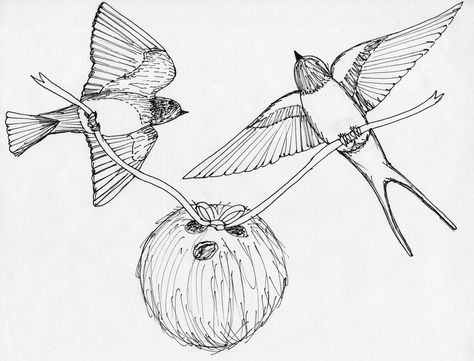
\includegraphics[width=0.7\linewidth]{img/swallows-coconut.jpg}
\end{center}
\end{frame}

\begin{frame}{Big, oversimplified history}
\vspace{-1.3 cm}
\begin{center}
\only<1>{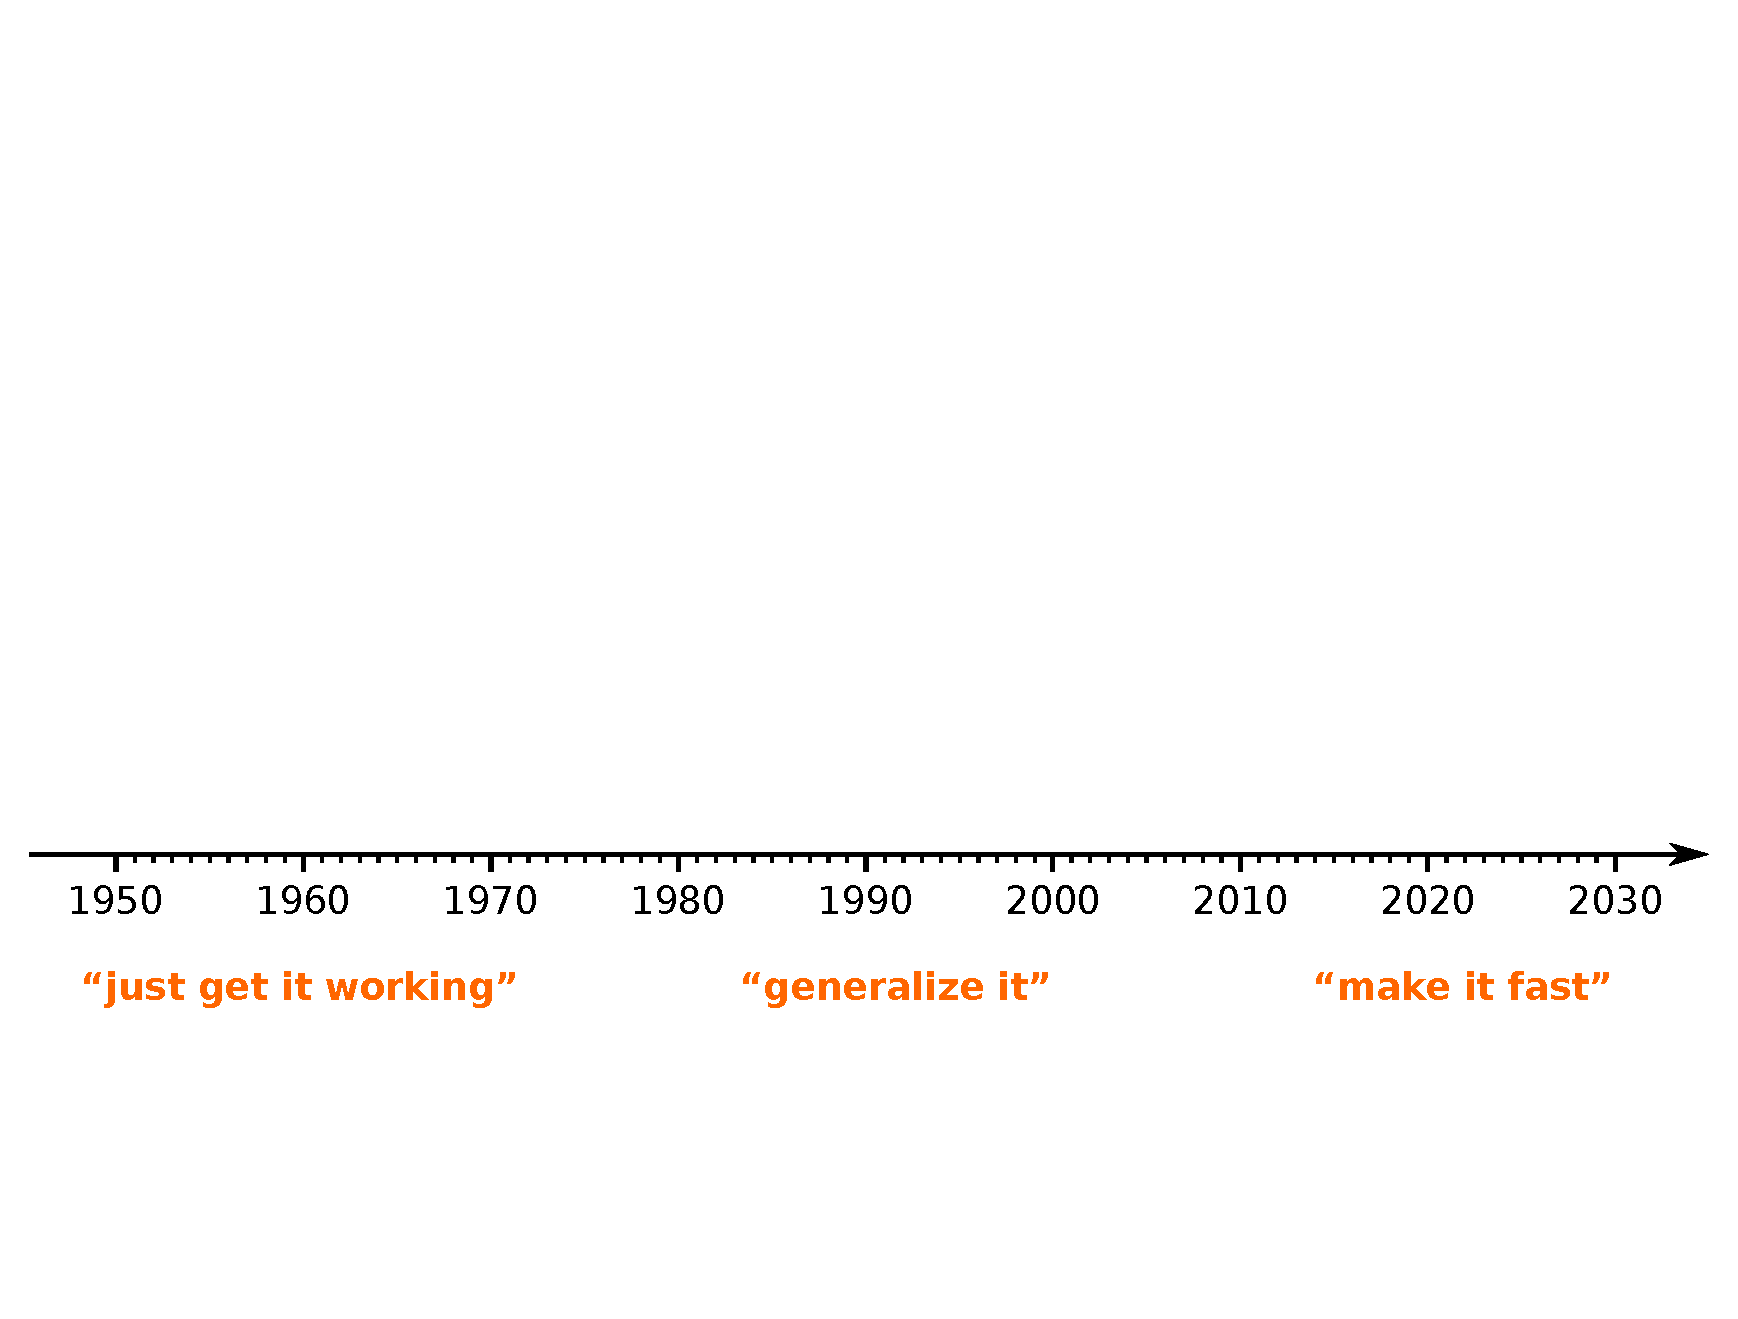
\includegraphics[width=0.88\linewidth]{img/big-oversimplfied-history-8.pdf}}\only<2>{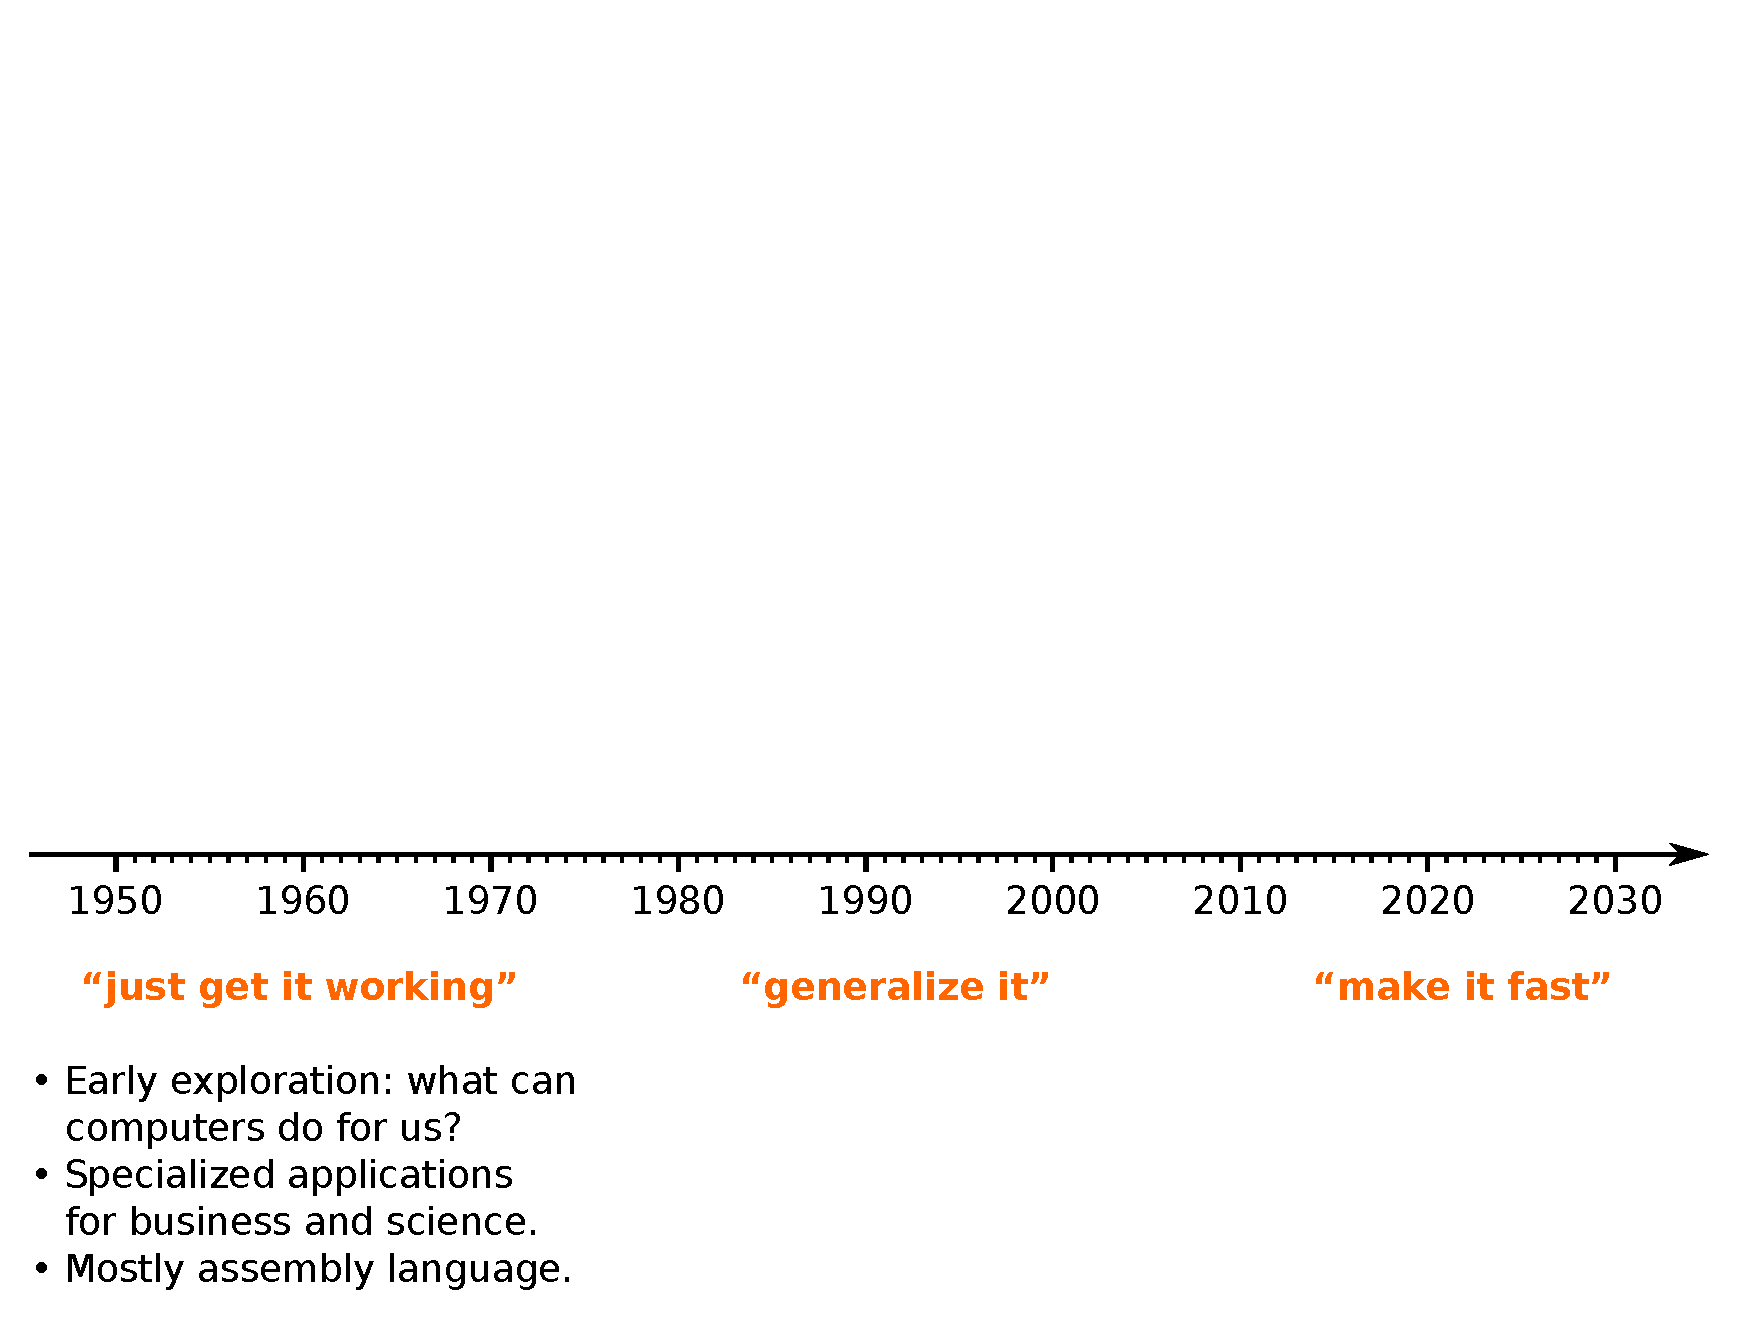
\includegraphics[width=0.88\linewidth]{img/big-oversimplfied-history-7.pdf}}\only<3>{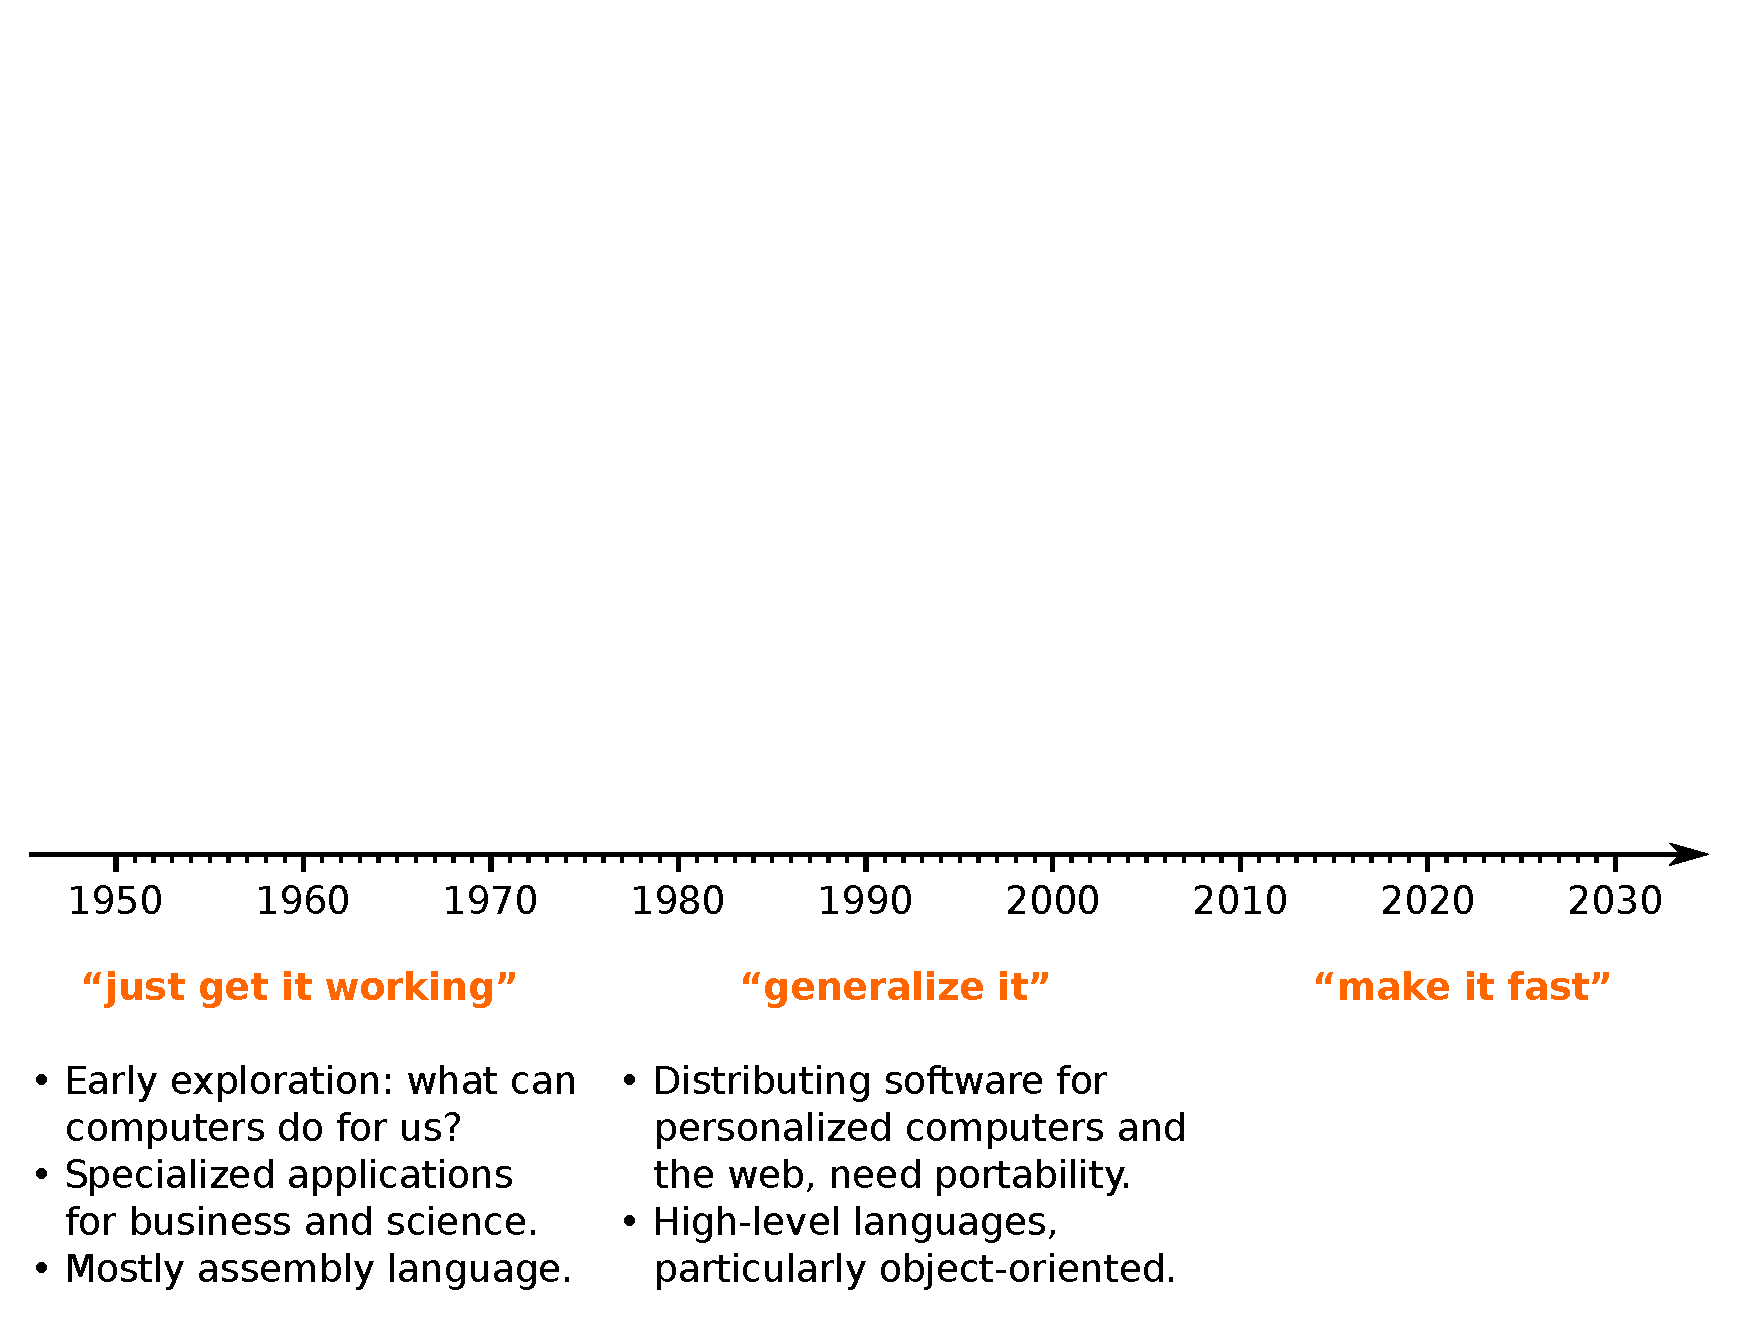
\includegraphics[width=0.88\linewidth]{img/big-oversimplfied-history-6.pdf}}\only<4>{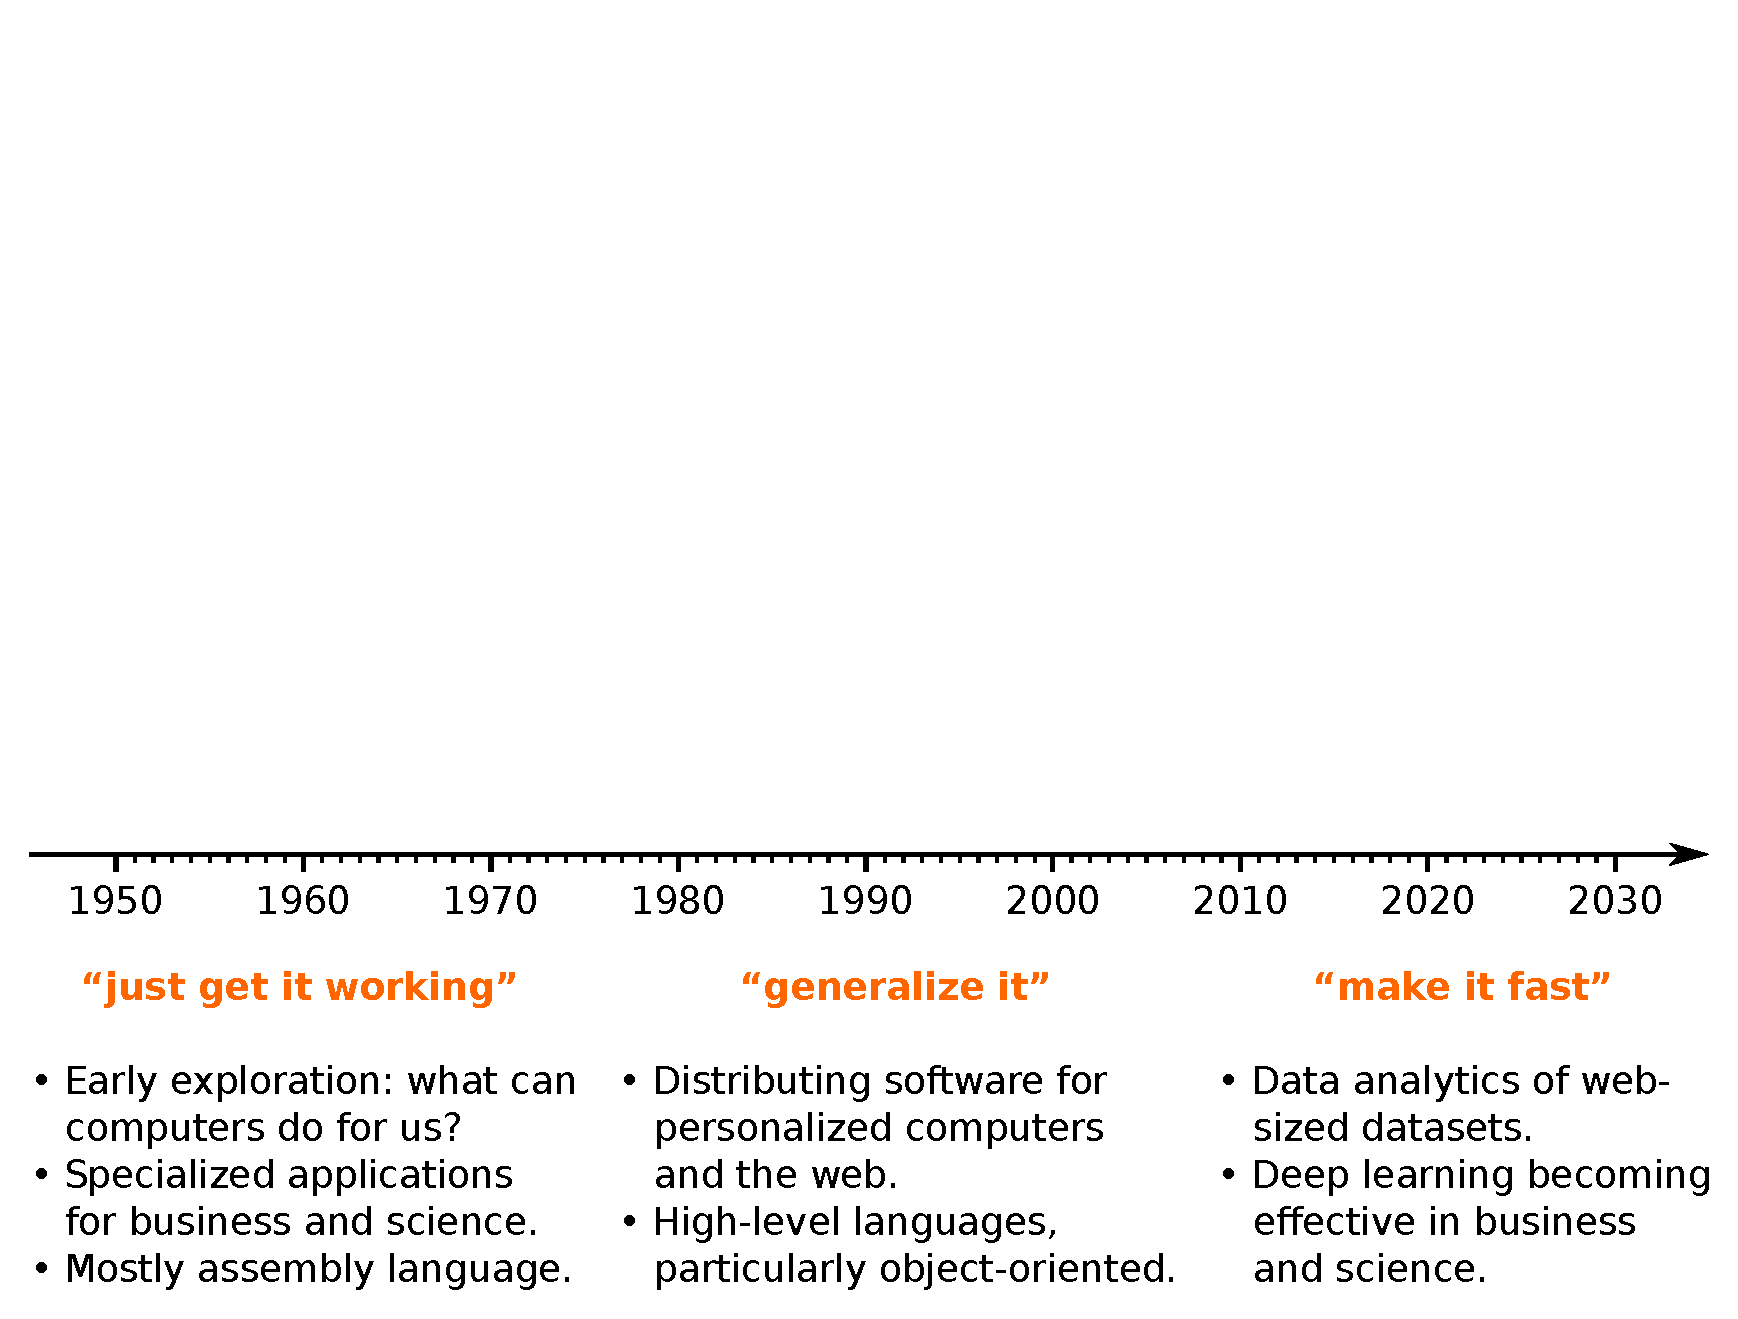
\includegraphics[width=0.88\linewidth]{img/big-oversimplfied-history-5.pdf}}\only<5>{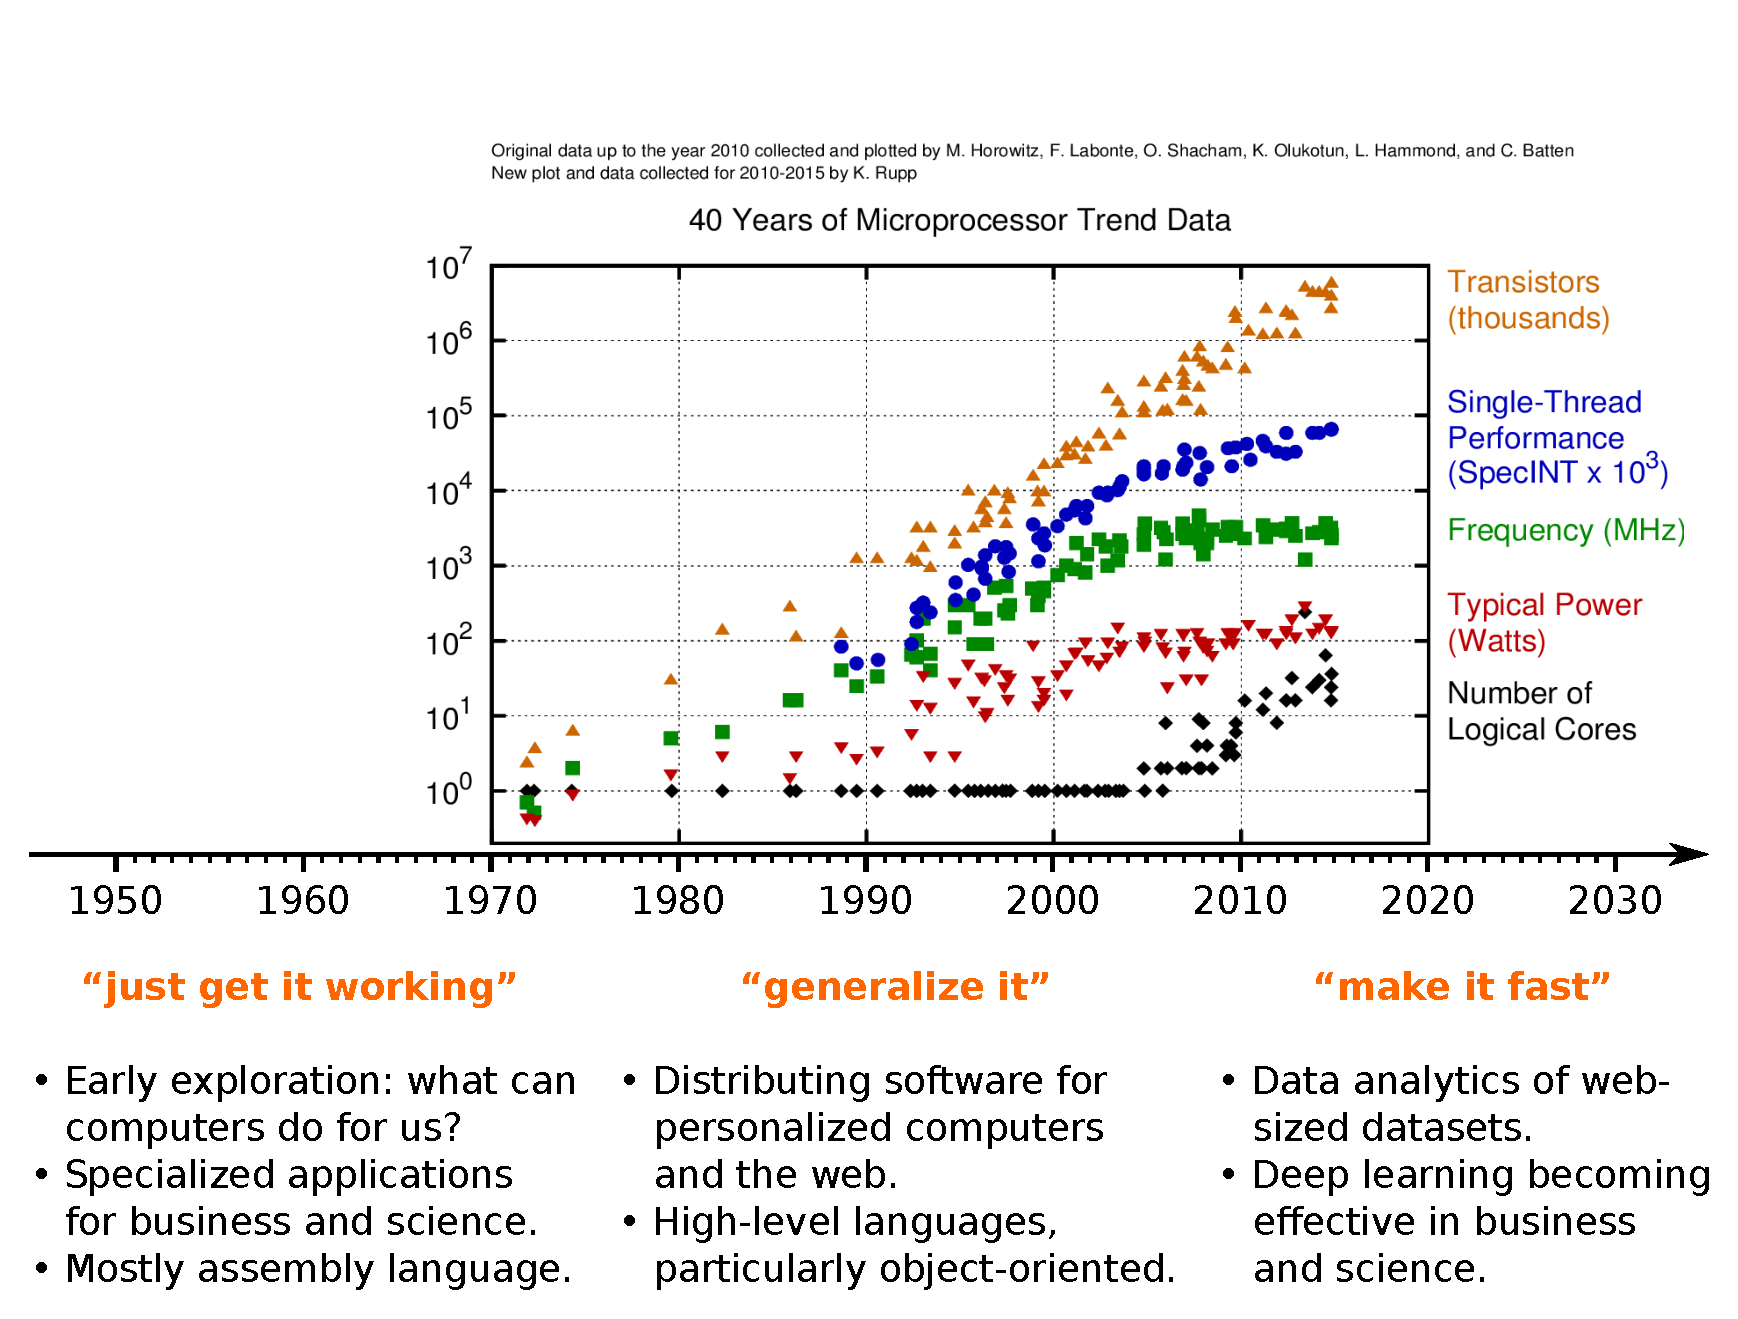
\includegraphics[width=0.88\linewidth]{img/big-oversimplfied-history-4.pdf}}\only<6>{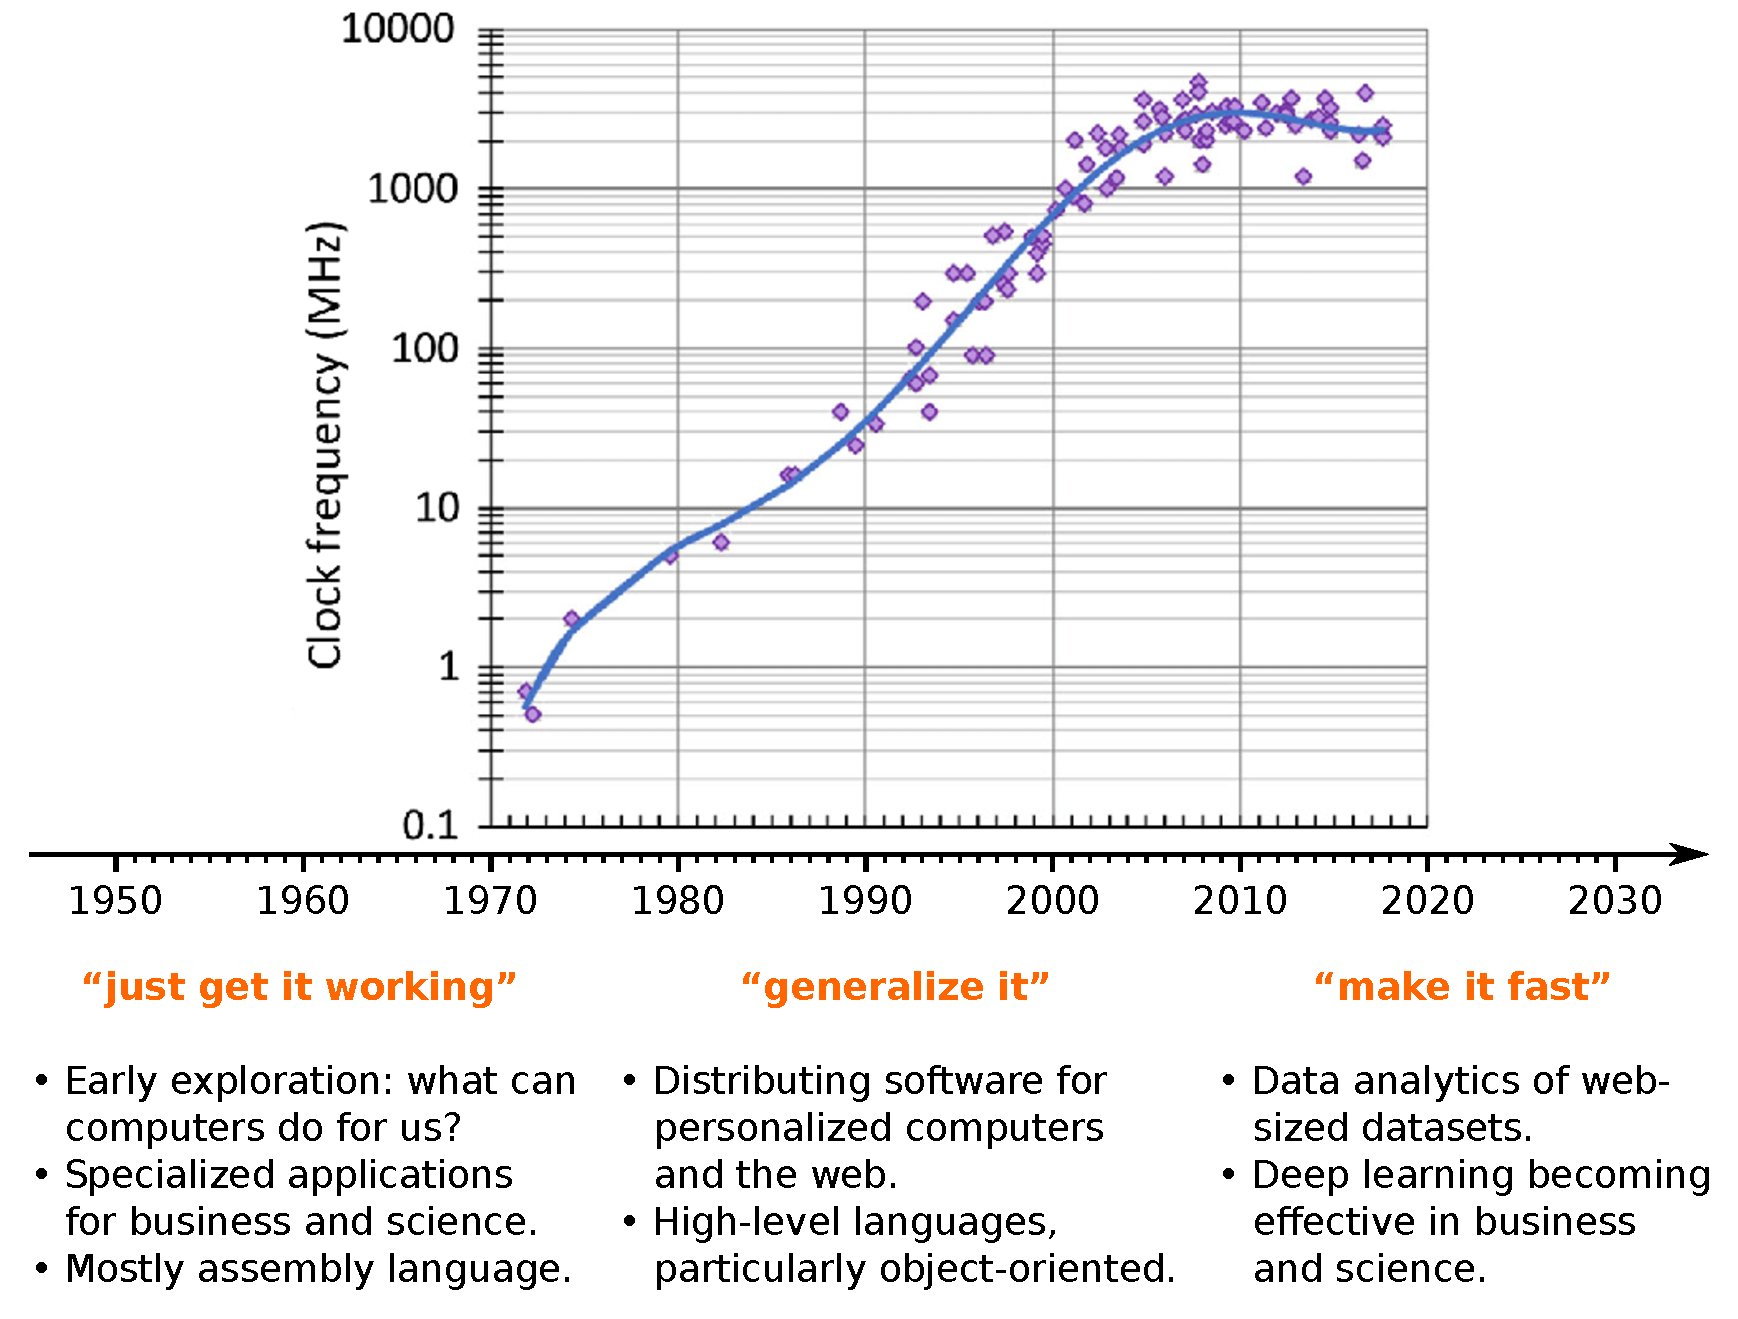
\includegraphics[width=0.88\linewidth]{img/big-oversimplfied-history-3.pdf}}\only<7>{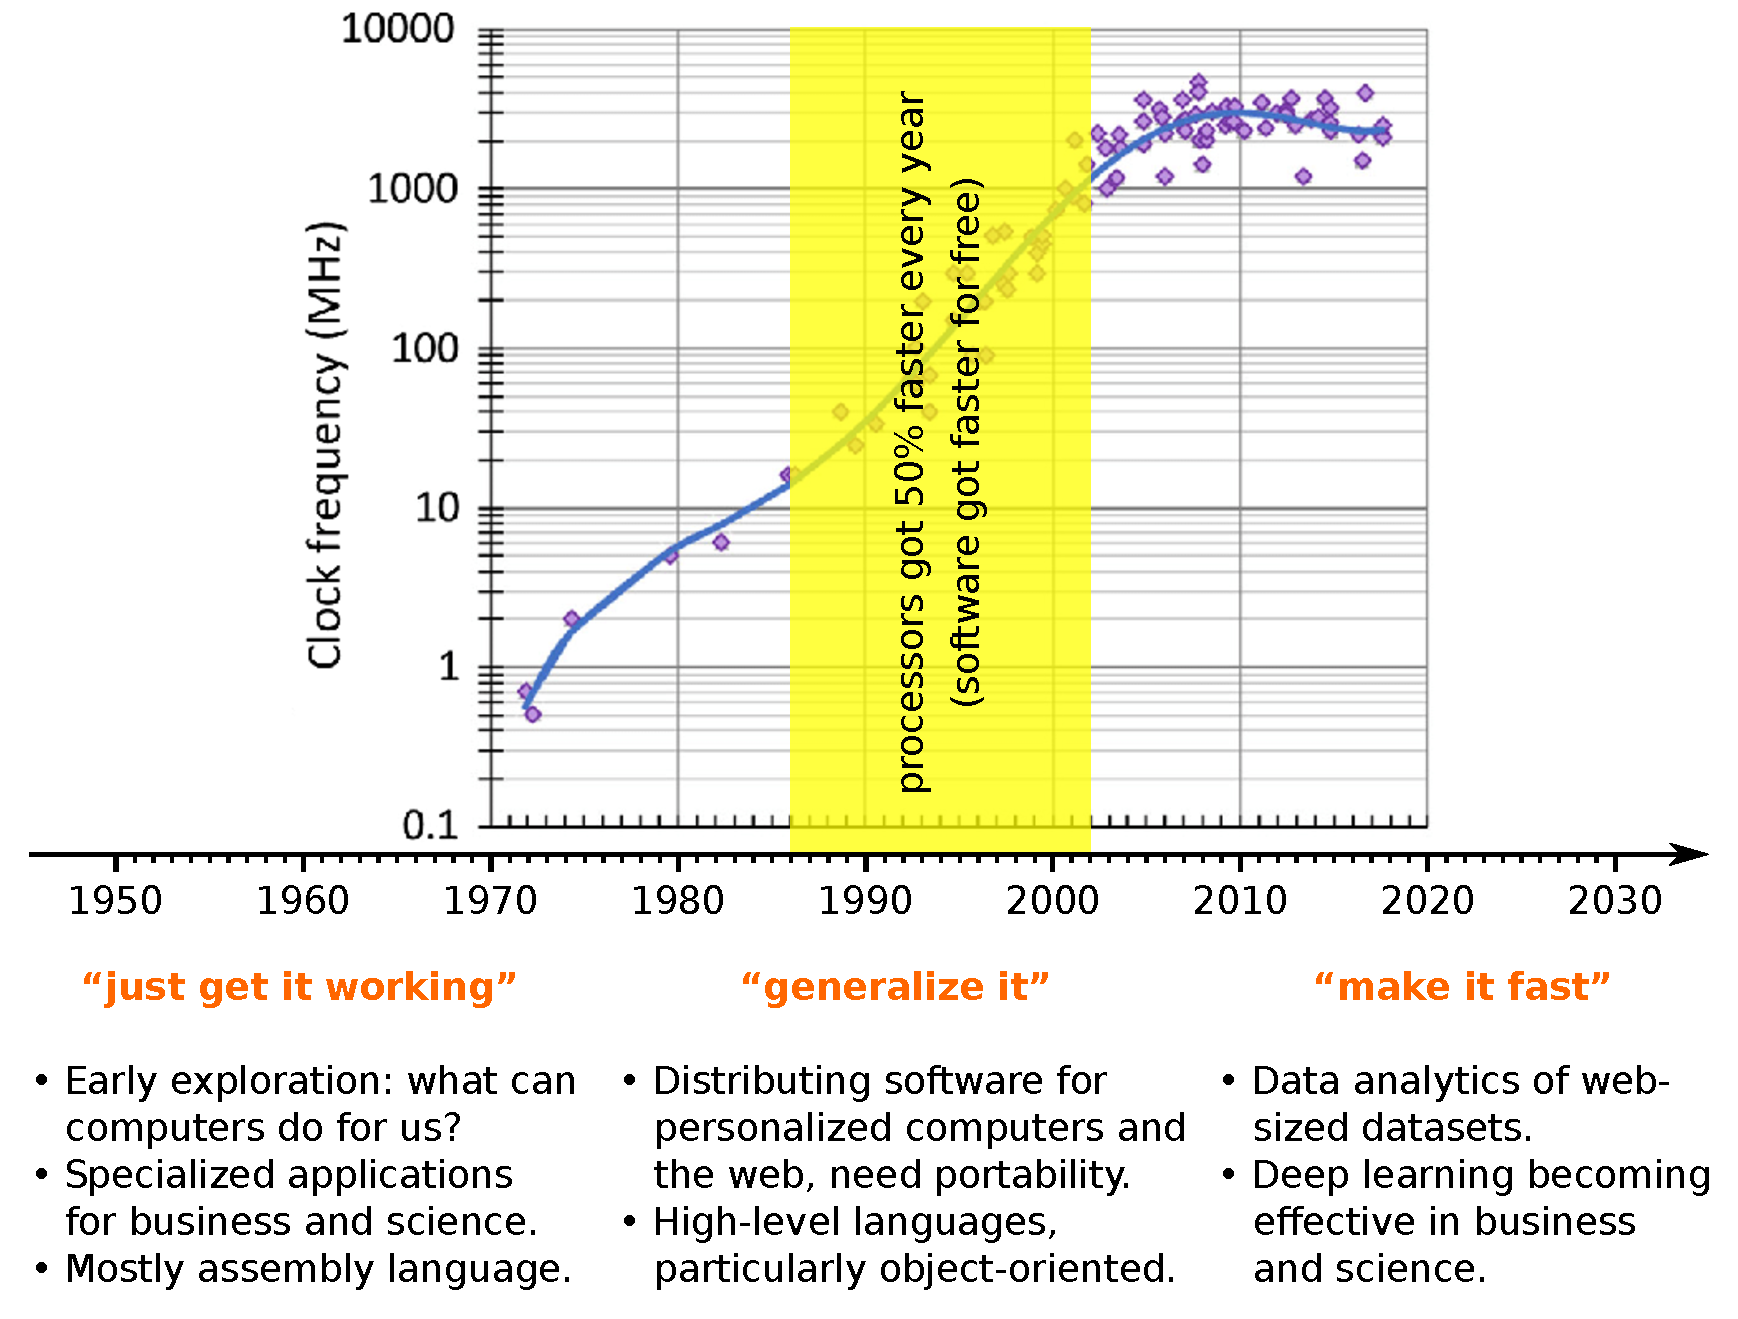
\includegraphics[width=0.88\linewidth]{img/big-oversimplfied-history-2.pdf}}\only<8>{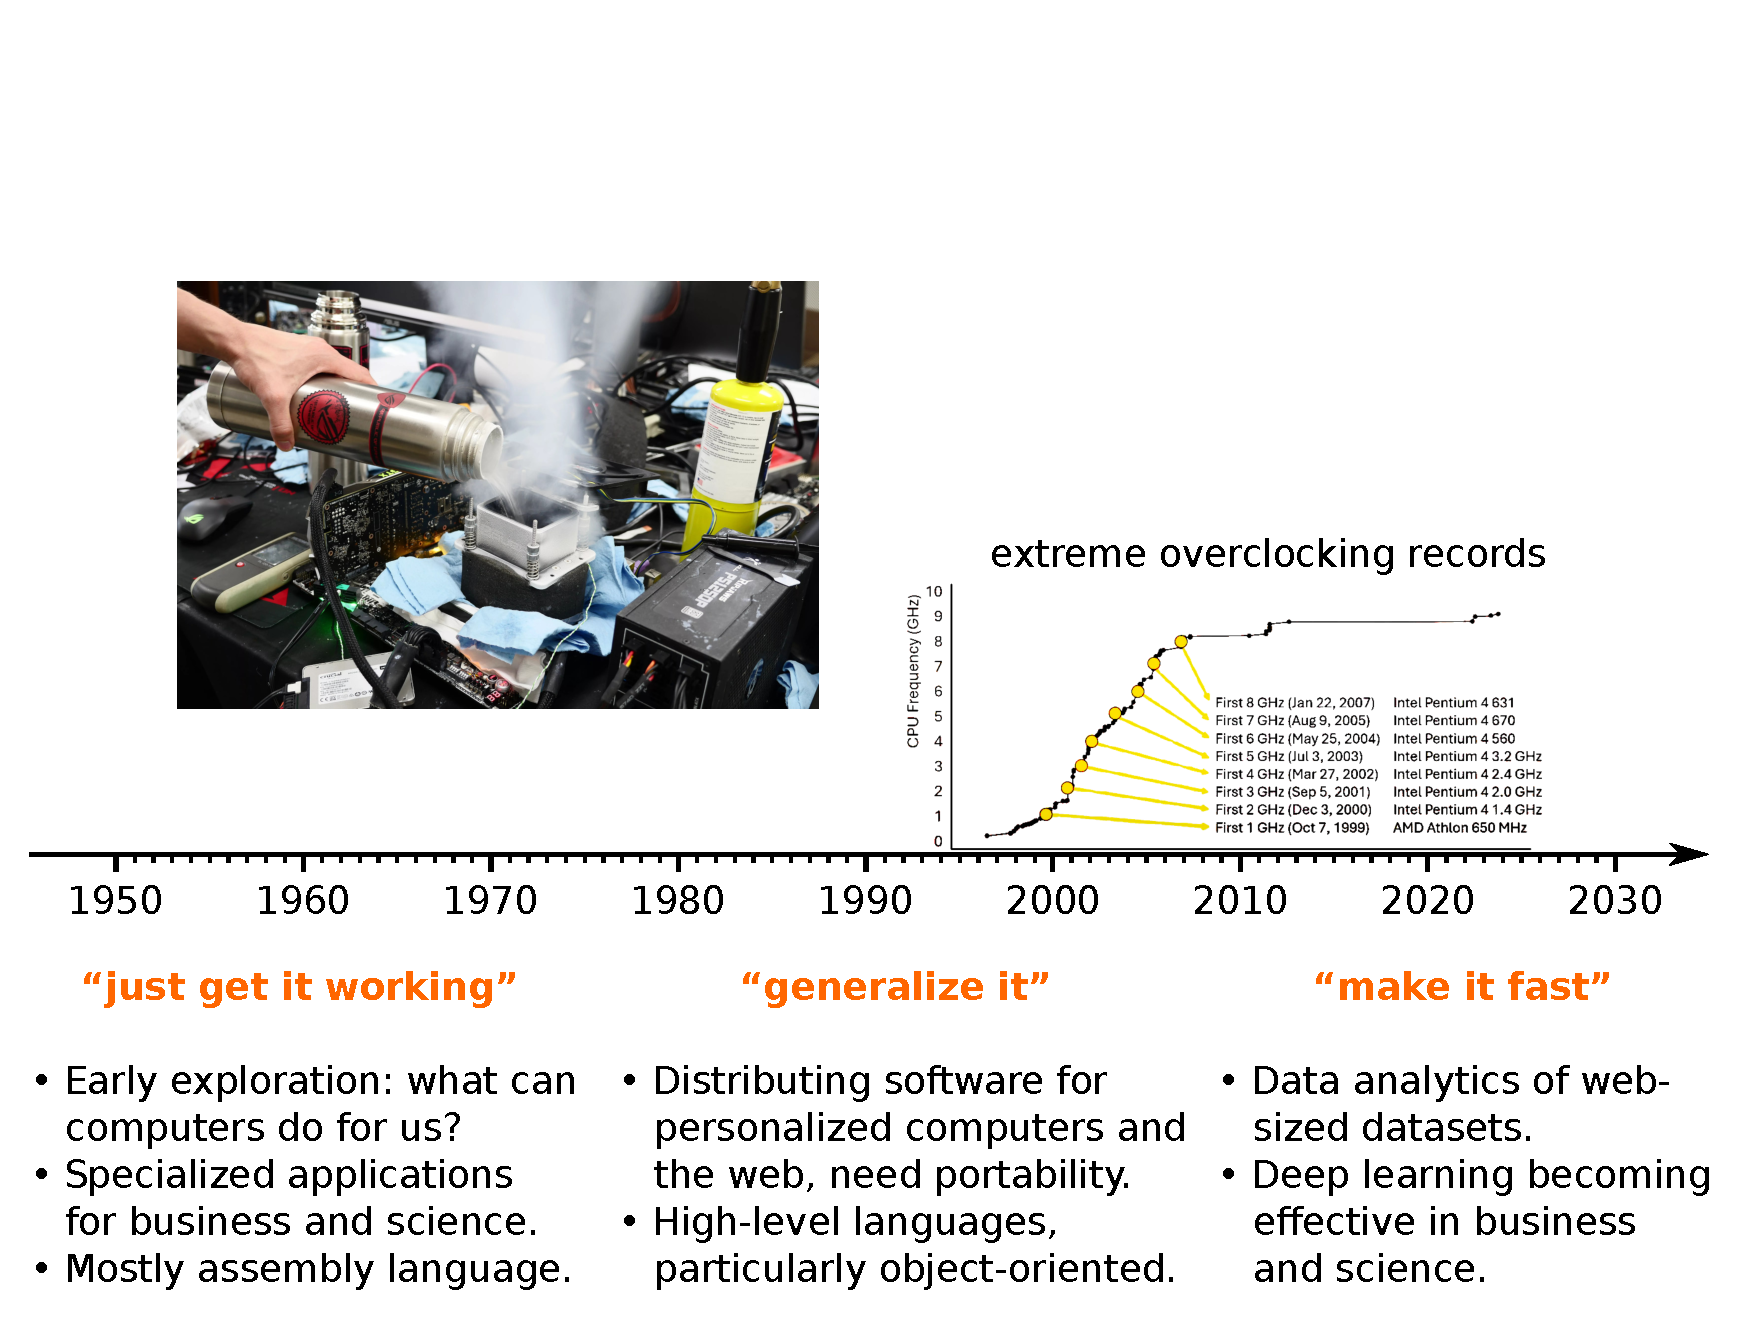
\includegraphics[width=0.88\linewidth]{img/big-oversimplfied-history-1.pdf}}
\end{center}
\end{frame}

\begin{frame}{\mbox{ }}
\LARGE
\begin{center}
\textcolor{darkblue}{Example of the change in mindset\ldots}
\end{center}
\end{frame}

\begin{frame}{Greg Owen's talk on Spark 2.0 (May 2016)}
\vspace{0.23 cm}
\begin{center}
\only<1>{
\includegraphics[width=0.95\linewidth]{img/greg-owen/page1.png}}\only<2>{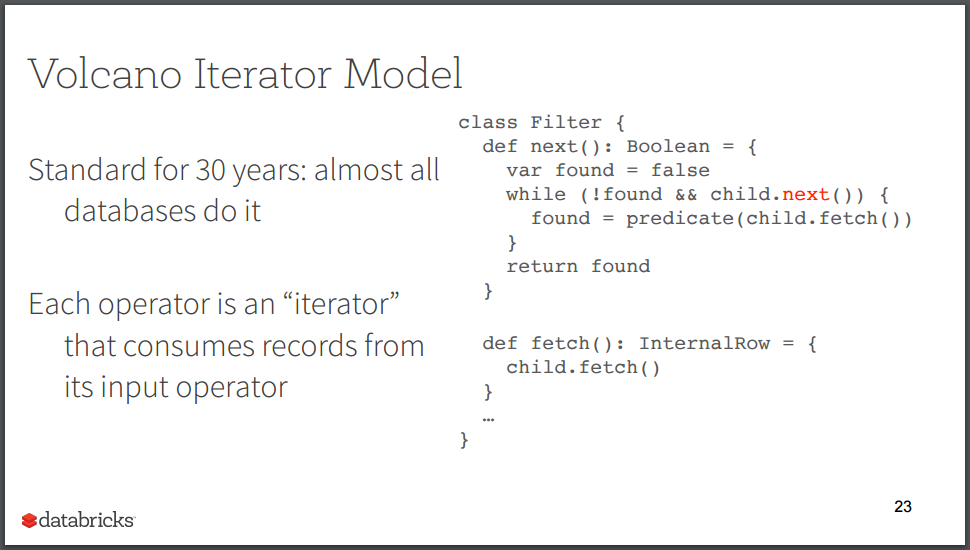
\includegraphics[width=0.95\linewidth]{img/greg-owen/page2.png}}\only<3>{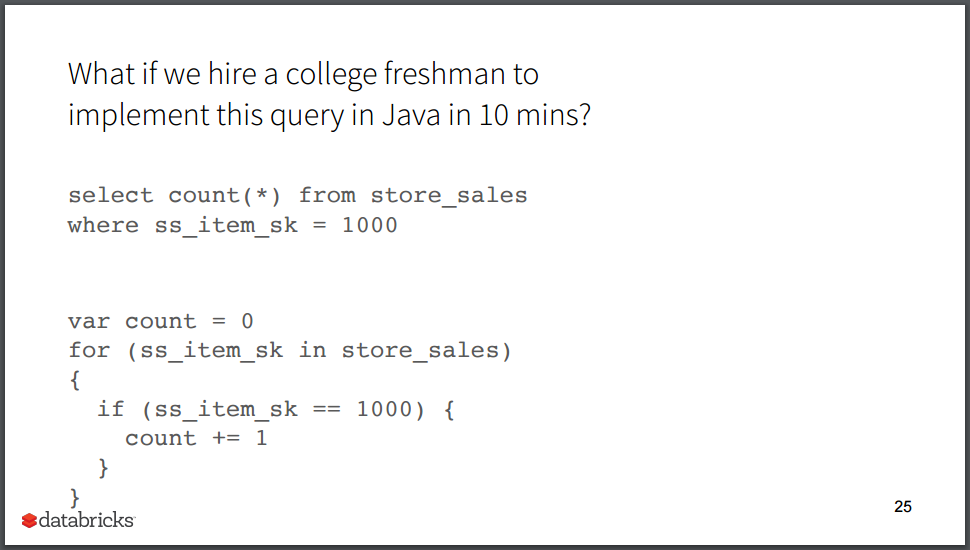
\includegraphics[width=0.95\linewidth]{img/greg-owen/page3.png}}\only<4>{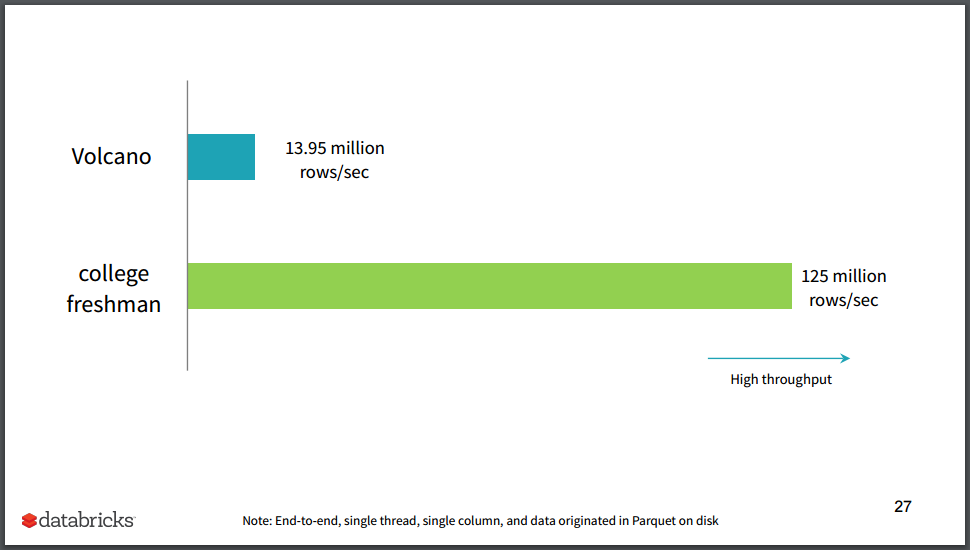
\includegraphics[width=0.95\linewidth]{img/greg-owen/page4.png}}\only<5>{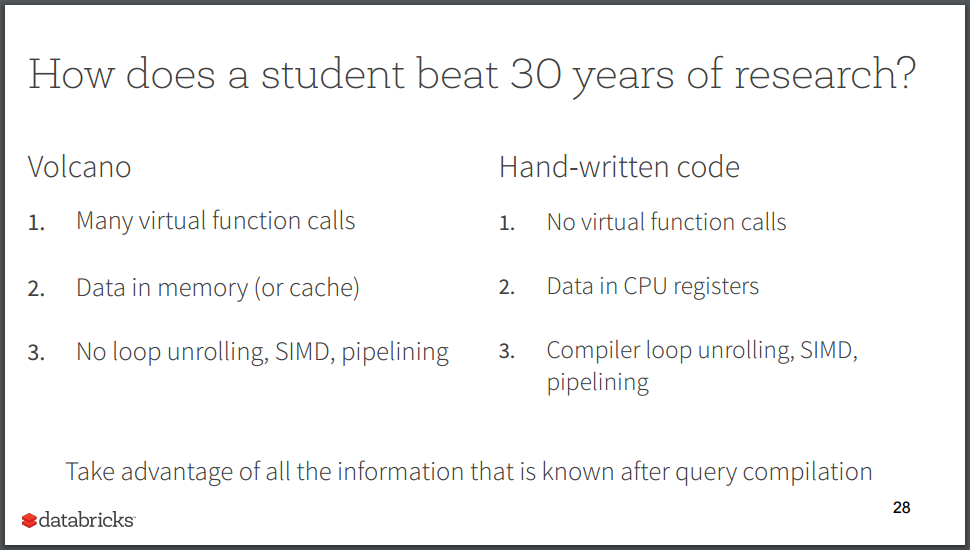
\includegraphics[width=0.95\linewidth]{img/greg-owen/page5.png}}
\end{center}
\end{frame}

\begin{frame}{\mbox{ }}
\vspace{0.5 cm}
\LARGE
\begin{center}
\textcolor{darkblue}{Tension between generalizability/portability and speed:}
\end{center}

\vspace{0.5 cm}
\large
\begin{columns}[t]
\column{0.4\linewidth}
\uncover<2->{We want to write generic, abstract code so that it can be used on a variety of computers and so that it can be remixed in other applications.}

\column{0.4\linewidth}
\uncover<3->{We want to write fast code so that we can analyze more data or perform more studies on it.}
\end{columns}

\Large
\vspace{0.5 cm}
\begin{center}
\uncover<4->{\textcolor{darkorange}{\bf Why can't we have it all?}}
\end{center}
\end{frame}

\begin{frame}{There is a such thing as a ``slow language.''}
\vspace{0.18 cm}
\begin{center}
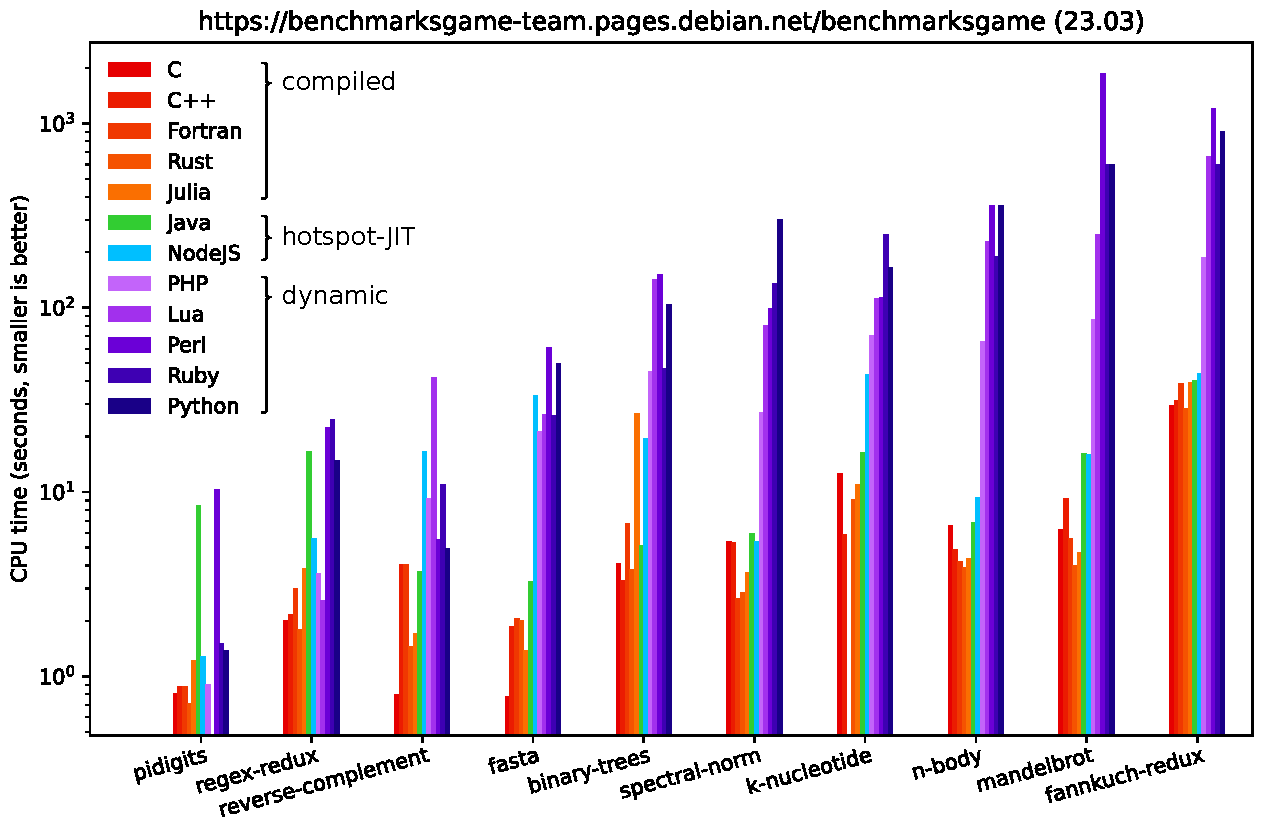
\includegraphics[width=0.85\linewidth]{img/benchmark-games-2023.pdf}
\end{center}
\end{frame}

\begin{frame}{\mbox{ }}
\vspace{0.1 cm}
\LARGE
\begin{center}
\textcolor{darkblue}{Languages with dynamic features make the computer do more things at runtime; those things take time.}
\end{center}

\vspace{0.1 cm}
\begin{center}
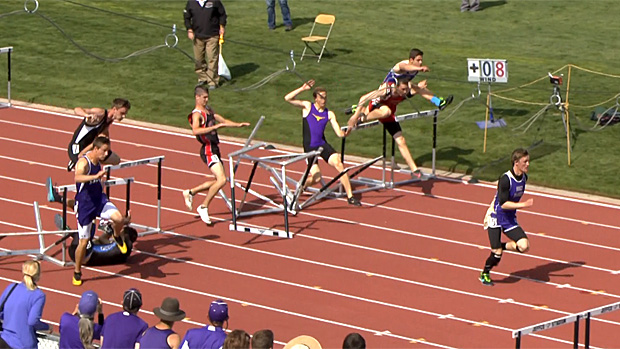
\includegraphics[width=0.7\linewidth]{img/hurdle9.jpg}
\end{center}
\end{frame}

\begin{frame}{Caveat}
\vspace{0.5 cm}
\Large
Some language features are static, compile-time abstractions, which provide generalizability/portability \underline{\it and} speed.

\vspace{0.25 cm}
\large
\begin{itemize}
\item<2-> Modern compilers are better at generating optimized machine code than most humans, taking full advantage of data locality, loop unrolling, SIMD vectorization, pipelining, etc.
\item<3-> Rust's borrow checker eliminates all memory leaks and double-free segfaults before the code runs, albeit by pointing them out and making the developer fix them manually.
\item<4-> Julia delays the compilation step, Just-In-Time or JIT-compilation, allowing developers to work with abstract code up to the point when it needs to run. (Many Python tools do this, too.)
\end{itemize}
\end{frame}

\begin{frame}{Dynamic language features}
\vspace{0.2 cm}
\begin{center}
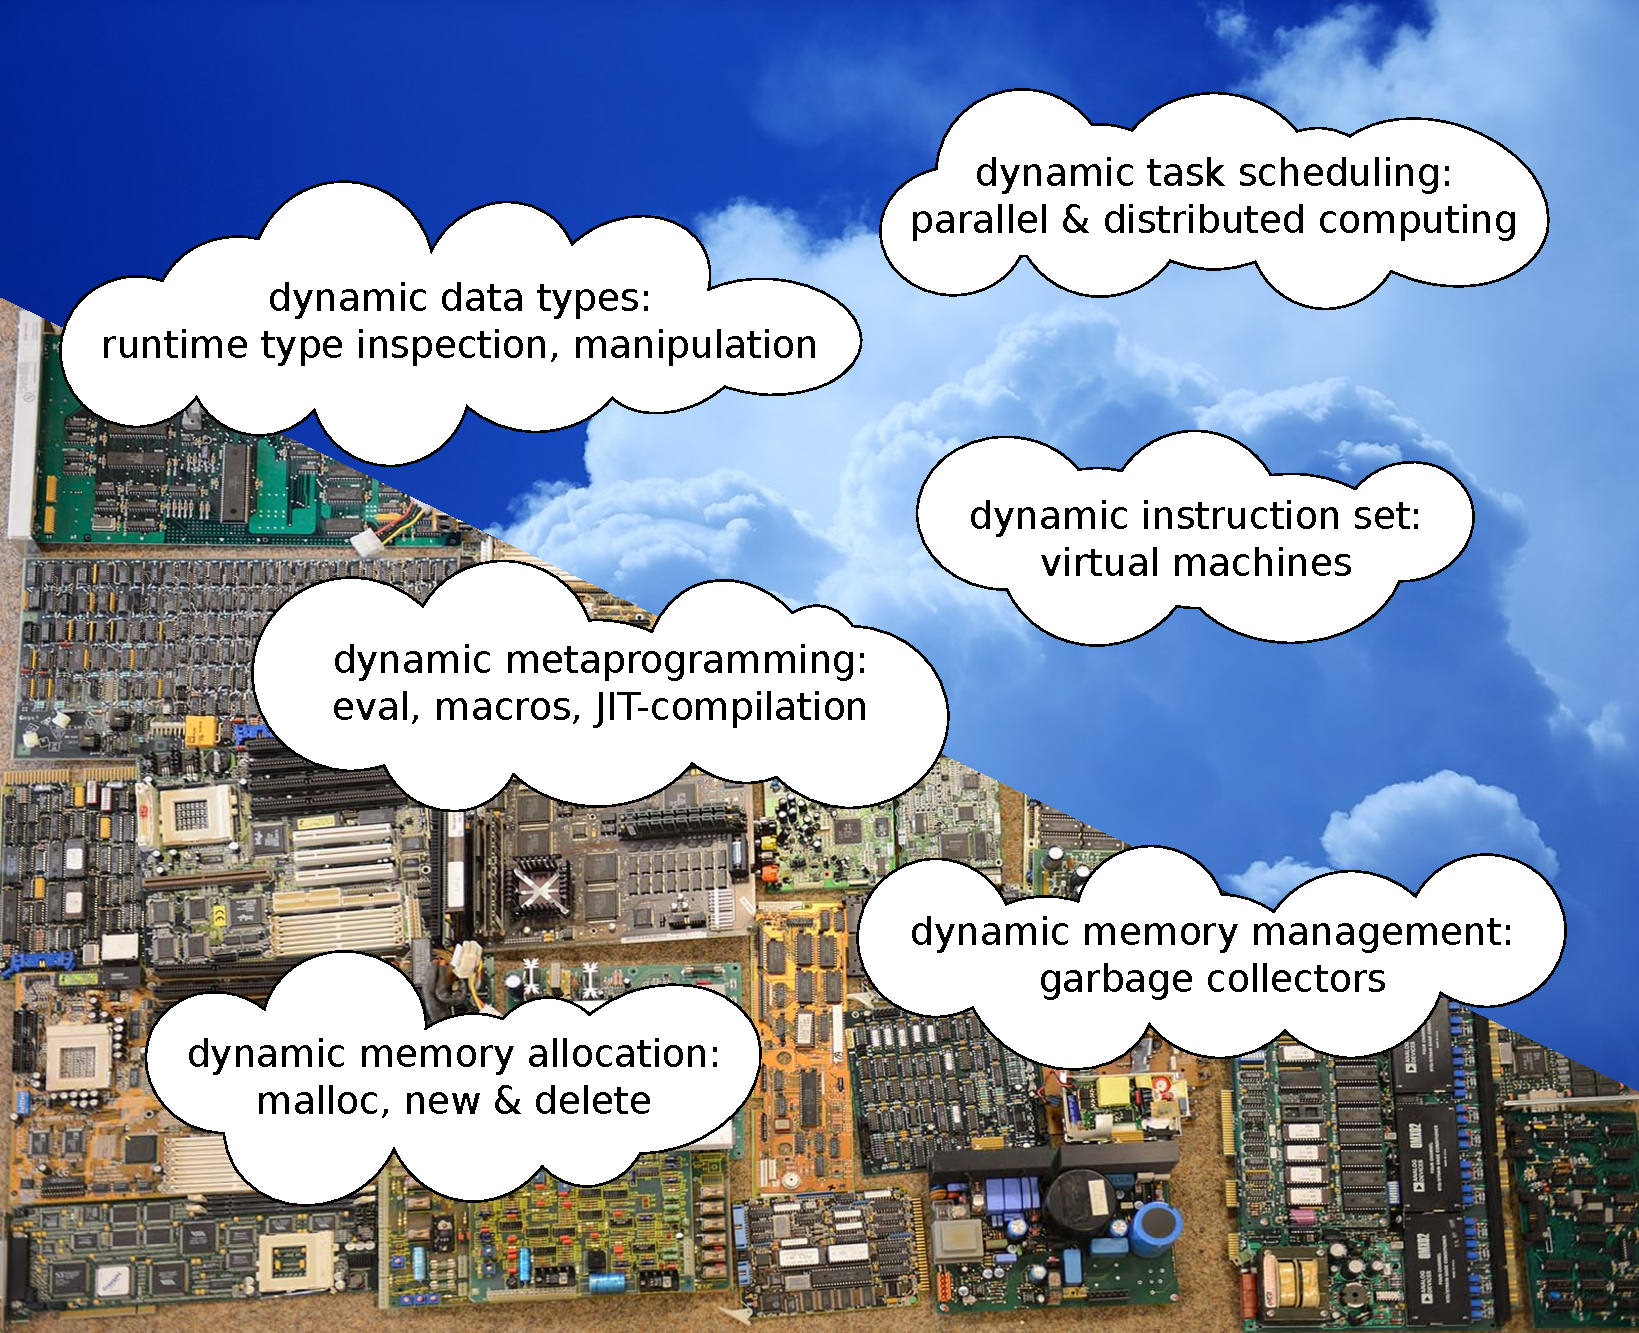
\includegraphics[width=0.67\linewidth]{img/dynamic-features.pdf}
\end{center}
\end{frame}

\begin{frame}{Dynamic language features}
\begin{columns}
\column{1.15\linewidth}
\begin{center}\renewcommand{\arraystretch}{1.25}
\begin{tabular}{l | c | c | c | c | c | c | c}
                     & alloc   & reference count              & GC      & eval    & VM      & type reflect & scheduling \\\hline
Fortran 77           &          &                                 &         &         &         &         &            \\
C                    & $\surd$  &                                 &         &         &         &         &            \\
C++                  & $\surd$  & {\small\mintinline{c++}{shared_ptr<T>}} &         &         &         & vtable only  & std library \\
C++ with ROOT        & $\surd$  & {\small\mintinline{c++}{shared_ptr<T>}} &         & $\surd$ &         & $\surd$ & $\surd$     \\
Rust                 & $\surd$  & {\small\mintinline{c++}{Rc<T>}}         &         &         &         & vtable only  & $\surd$ \\
Swift                & $\surd$  & $\surd$                         &         &         &         & vtable only  & $\surd$     \\
Julia                & $\surd$  &                                 & $\surd$ & $\surd$ &         & $\surd$ & std macros  \\
Go                   & $\surd$  &                                 & $\surd$ &         &         & vtable only  & $\surd$     \\
Java (JVM languages) & $\surd$  &                                 & $\surd$ &         & $\surd$ & $\surd$ & std library \\
Lua                  & $\surd$  &                                 & $\surd$ & $\surd$ & $\surd$ & $\surd$ &             \\
Python               & $\surd$  & $\surd$                         & $\surd$ & $\surd$ & $\surd$ & $\surd$ & $\surd$     \\
\end{tabular}
\end{center}
\end{columns}
\end{frame}

\begin{frame}{Why use a language with these dynamic features, anyway?}
\vspace{0.35 cm}
\begin{center}
\only<1>{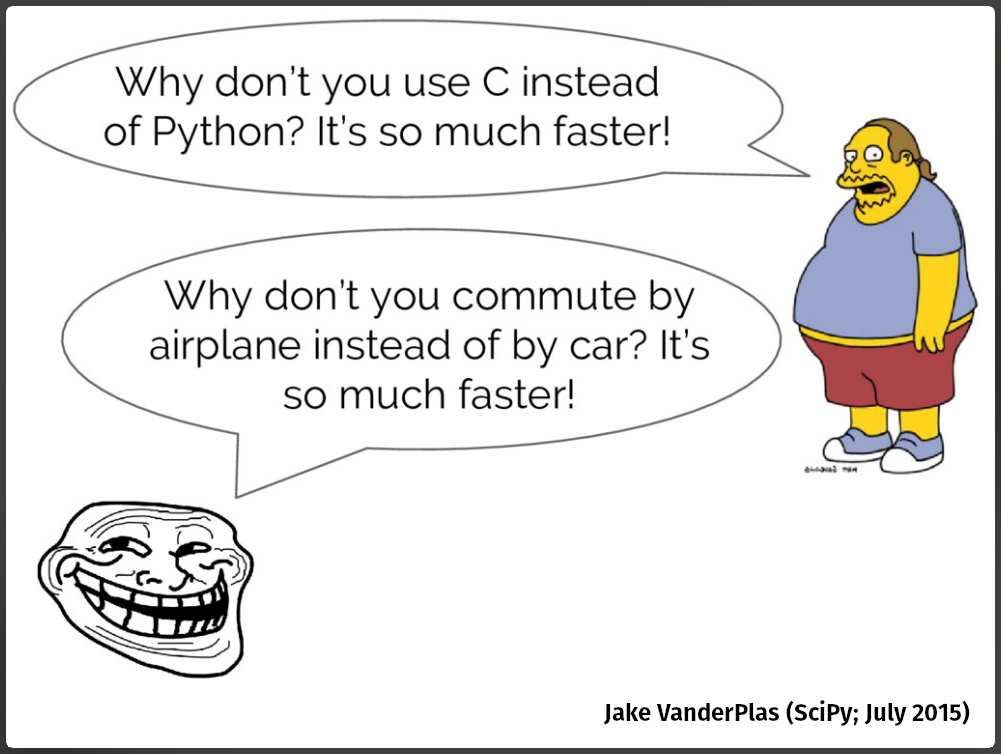
\includegraphics[width=0.7\linewidth]{img/commute-by-plane.png}}\only<2>{\vspace{-0.2 cm}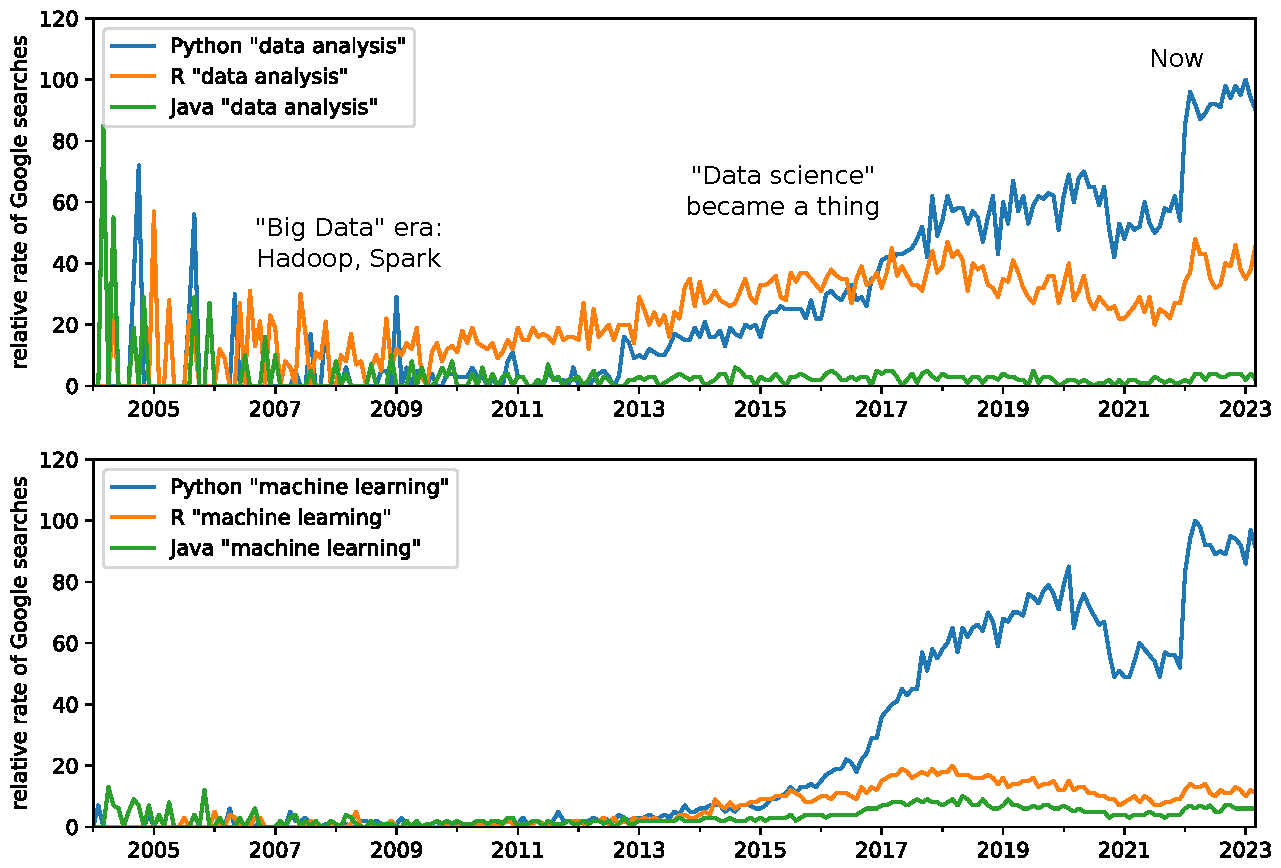
\includegraphics[width=0.8\linewidth]{img/analytics-by-language.pdf}}
\end{center}
\end{frame}

\begin{frame}{\mbox{ }}
\LARGE
\begin{center}
\textcolor{darkblue}{Dynamic language features are for \underline{\it developers!}}
\end{center}

\vspace{0.3 cm}
\large
\begin{itemize}\setlength{\itemsep}{0.2 cm}
\item<2-> \textcolor{darkblue}{malloc, new \& delete:} make objects on the fly, arbitrary graph relationships
\item<3-> \textcolor{darkblue}{garbage collectors:} eliminate all memory leaks and double-free segfaults
\item<4-> \textcolor{darkblue}{eval, macros, JIT-compilation:} deal with information that arrives ``late''
\item<5-> \textcolor{darkblue}{virtual machines:} portability across hardware architectures
\item<6-> \textcolor{darkblue}{runtime type inspection, manipulation:} make runtime choices based on types
\item<7-> \textcolor{darkblue}{parallel \& distributed computing abstractions:} let a scheduler worry about ordering tasks by data dependencies
\end{itemize}
\end{frame}

\begin{frame}{\mbox{ }}
\LARGE
\begin{center}
\textcolor{darkblue}{In scientific programming and data analysis, \\ the developer \underline{\it is} the user.}

\vspace{1 cm}
\uncover<2->{\textcolor{darkblue}{The time it takes you to write the code \\ is part of the optimization.}}

\end{center}
\end{frame}

\begin{frame}{Long history of attempts to use fast compiled code in Python}
\vspace{0.25 cm}
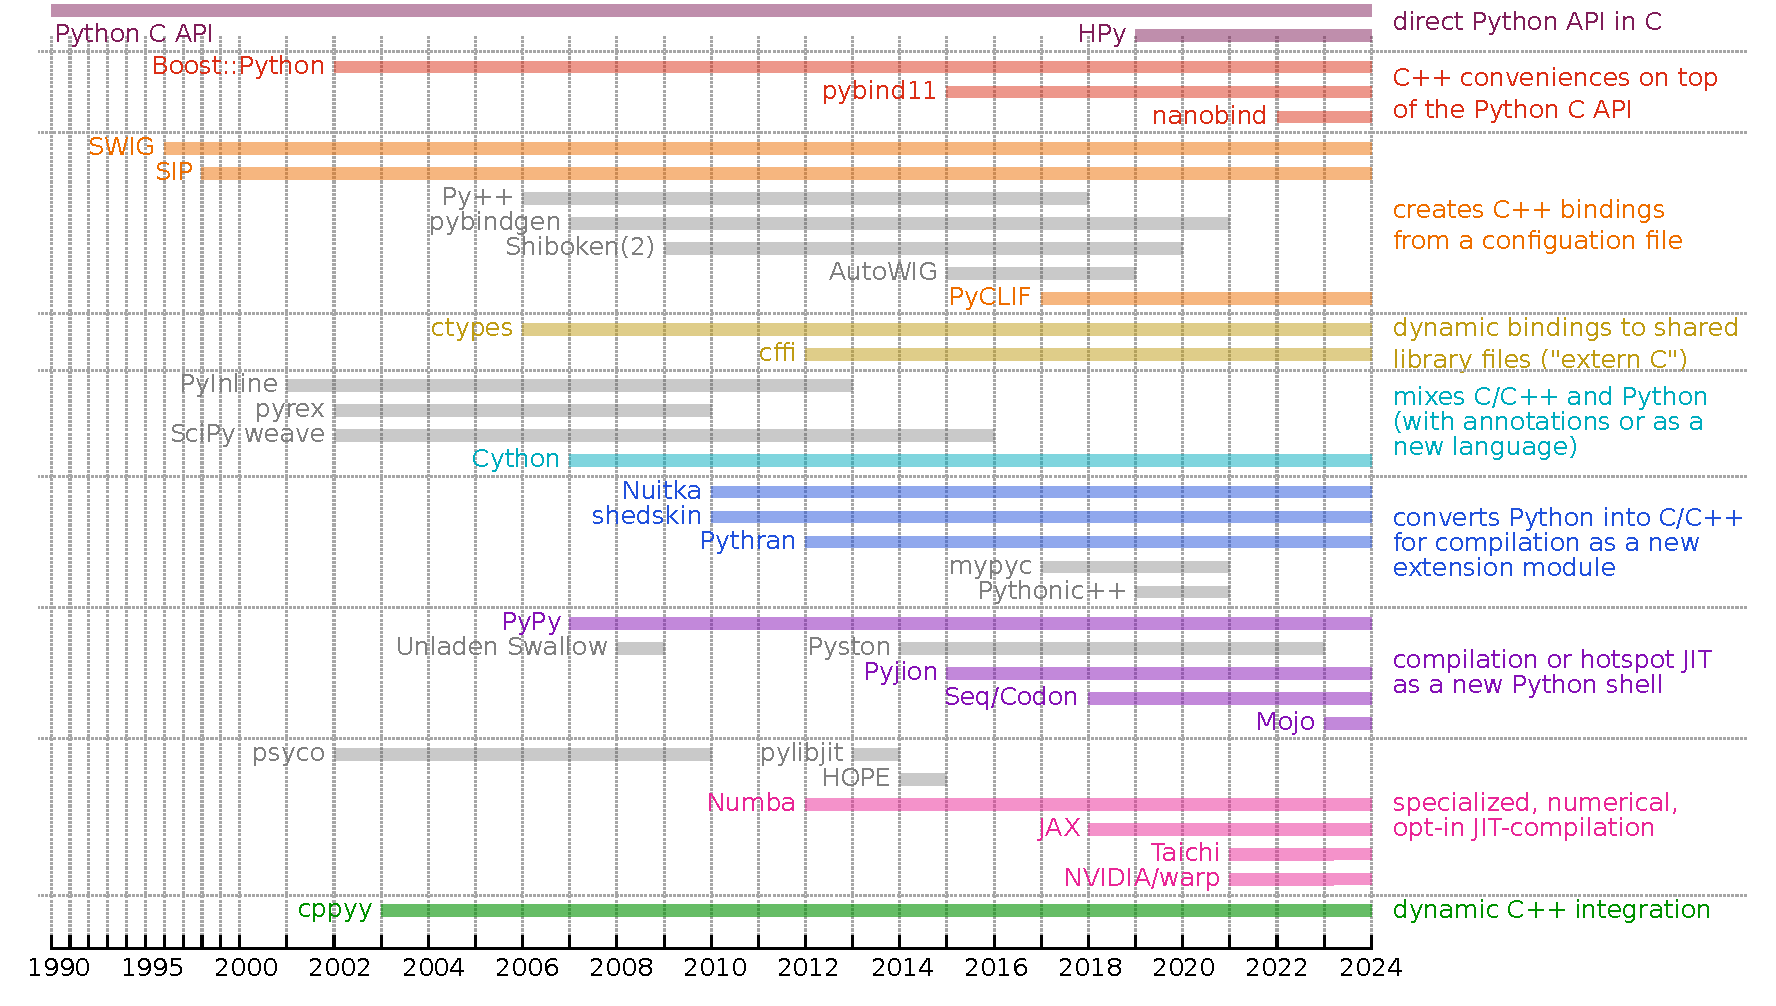
\includegraphics[width=\linewidth]{img/history-of-bindings-2.pdf}
\end{frame}

\begin{frame}{\mbox{ }}
\LARGE
\begin{center}
\textcolor{darkblue}{This week, you'll see how to use dynamic features \\ when useful and how to avoid them when necessary.}
\end{center}
\end{frame}

\begin{frame}[fragile]{\mbox{ }}
\LARGE
\begin{center}
\textcolor{darkblue}{But first, let's see what an implementation looks like.}
\end{center}

\vspace{1 cm}
\scriptsize
\begin{verbatim}
% c++ -std=c++11 -O3 baby-python.cpp -o baby-python
% ./baby-python 
                     num = -123        add(x, x)   get(lst, i)   map(f, lst)
               oo    lst = [1, 2, 3]   mul(x, x)   len(lst)      reduce(f, lst)
. . . __/\_/\_/`'    f = def(x) single-expr   f = def(x, y) { ... ; last-expr }

>>
\end{verbatim}
\end{frame}

\begin{frame}{\mbox{ }}
\LARGE
\begin{center}
\textcolor{darkblue}{\bf BACKUP}
\end{center}
\end{frame}

\begin{frame}{\mbox{ }}
\vspace{0.5 cm}
\begin{center}
\only<1>{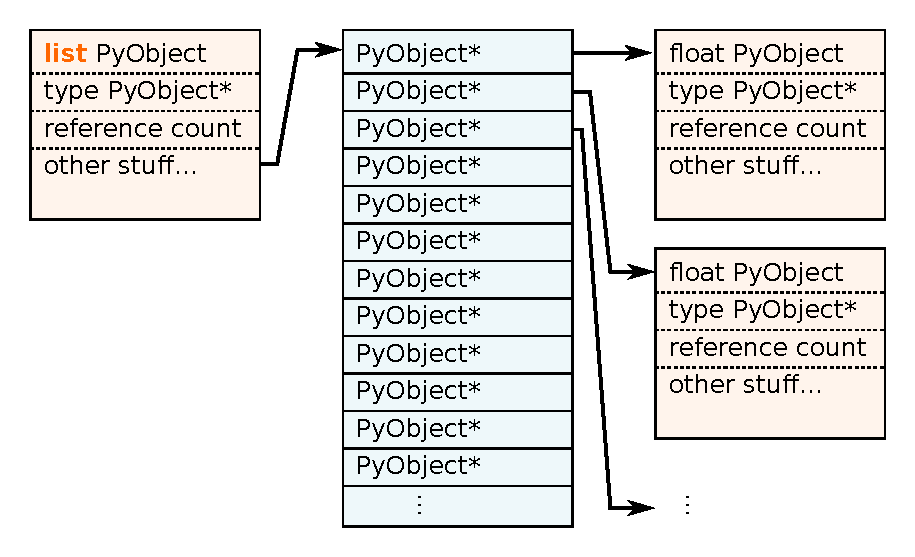
\includegraphics[width=0.8\linewidth]{img/python-list-layout.pdf}}\only<2>{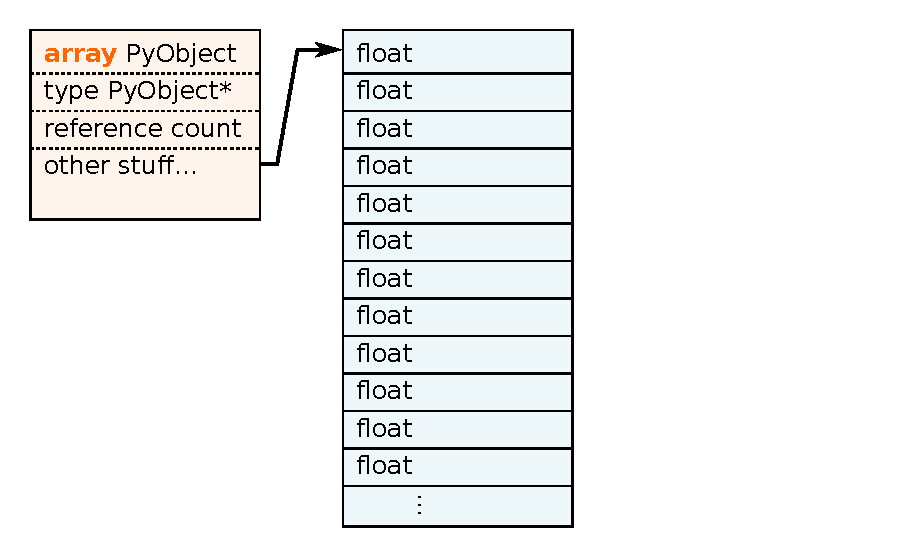
\includegraphics[width=0.8\linewidth]{img/python-array-layout.pdf}}
\end{center}
\end{frame}

\begin{frame}{\mbox{ }}
\begin{center}
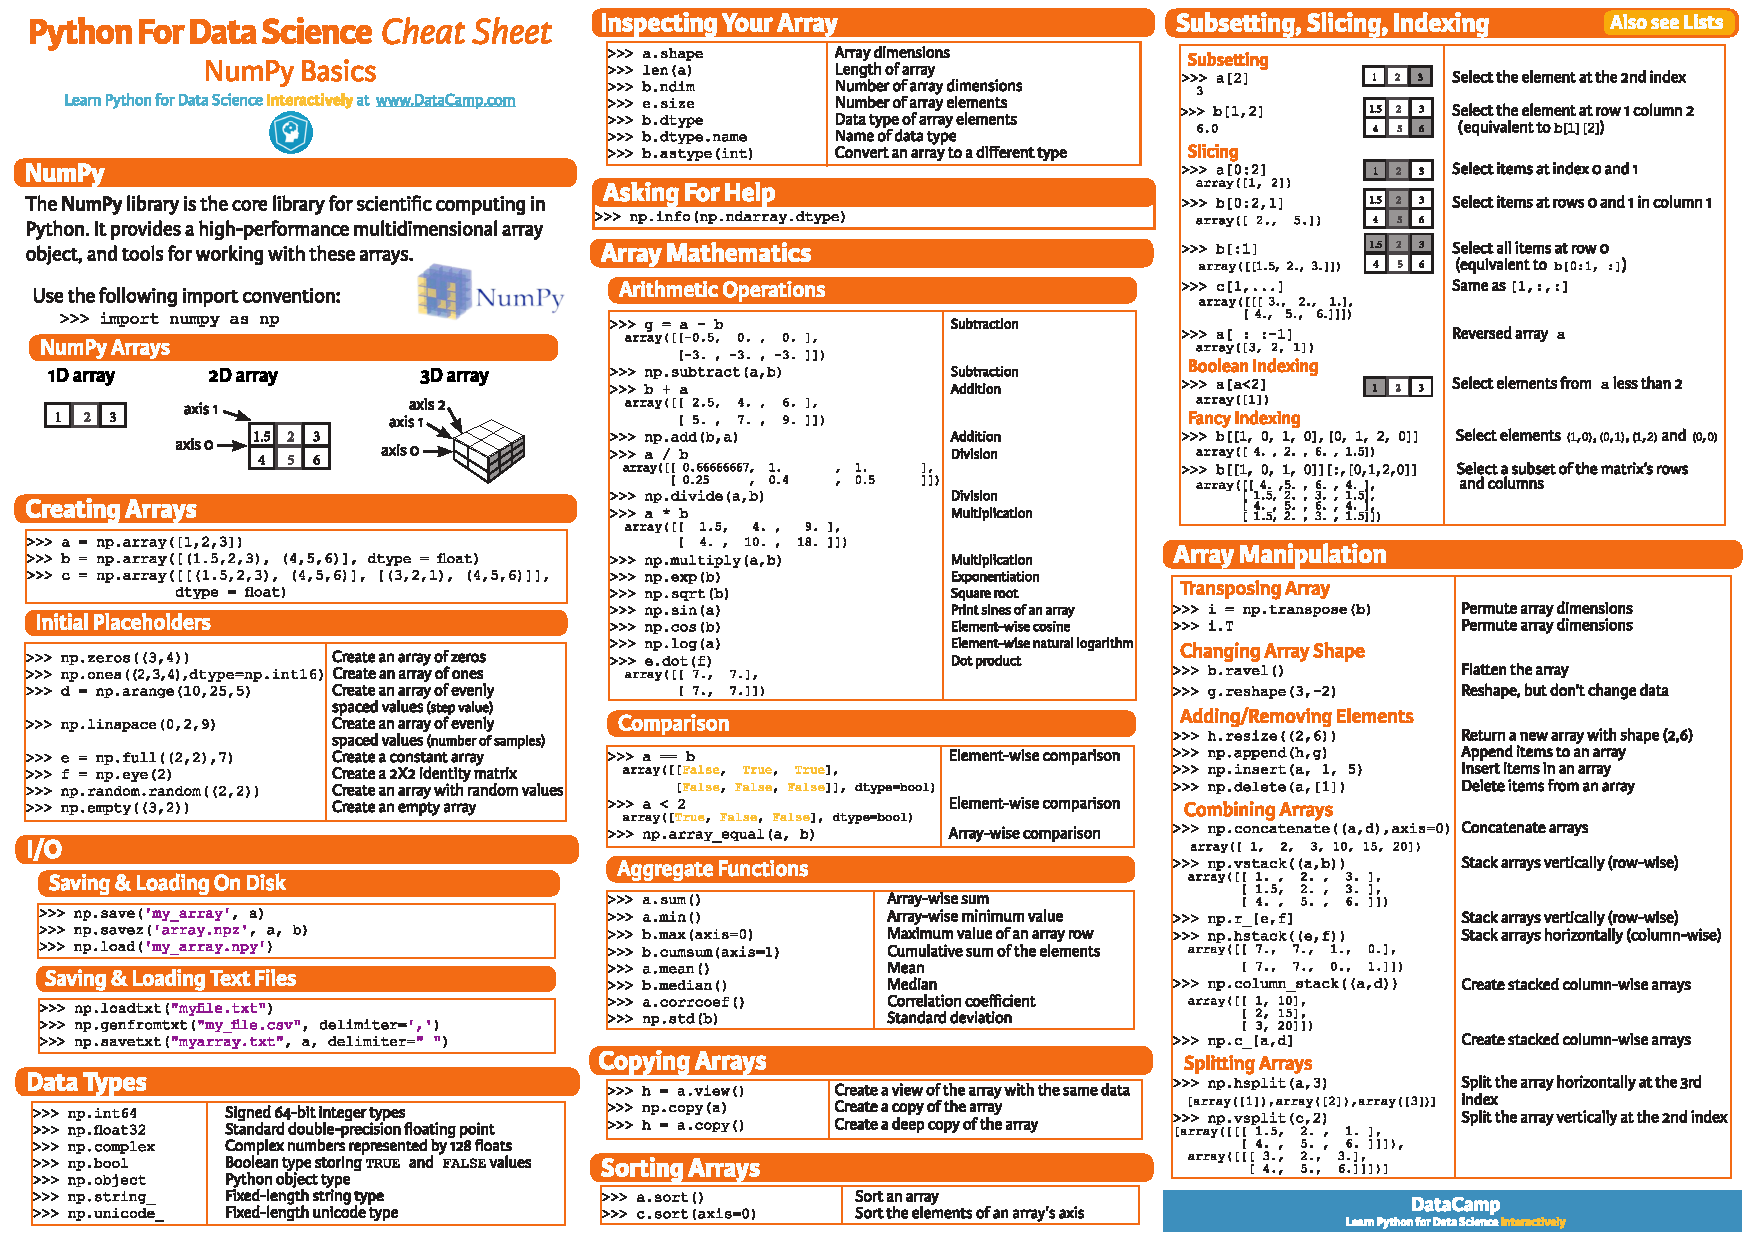
\includegraphics[width=0.8\linewidth]{img/Numpy_Python_Cheat_Sheet.pdf}
\end{center}
\end{frame}

\begin{frame}{\mbox{ }}
\vspace{0.5 cm}
\begin{center}
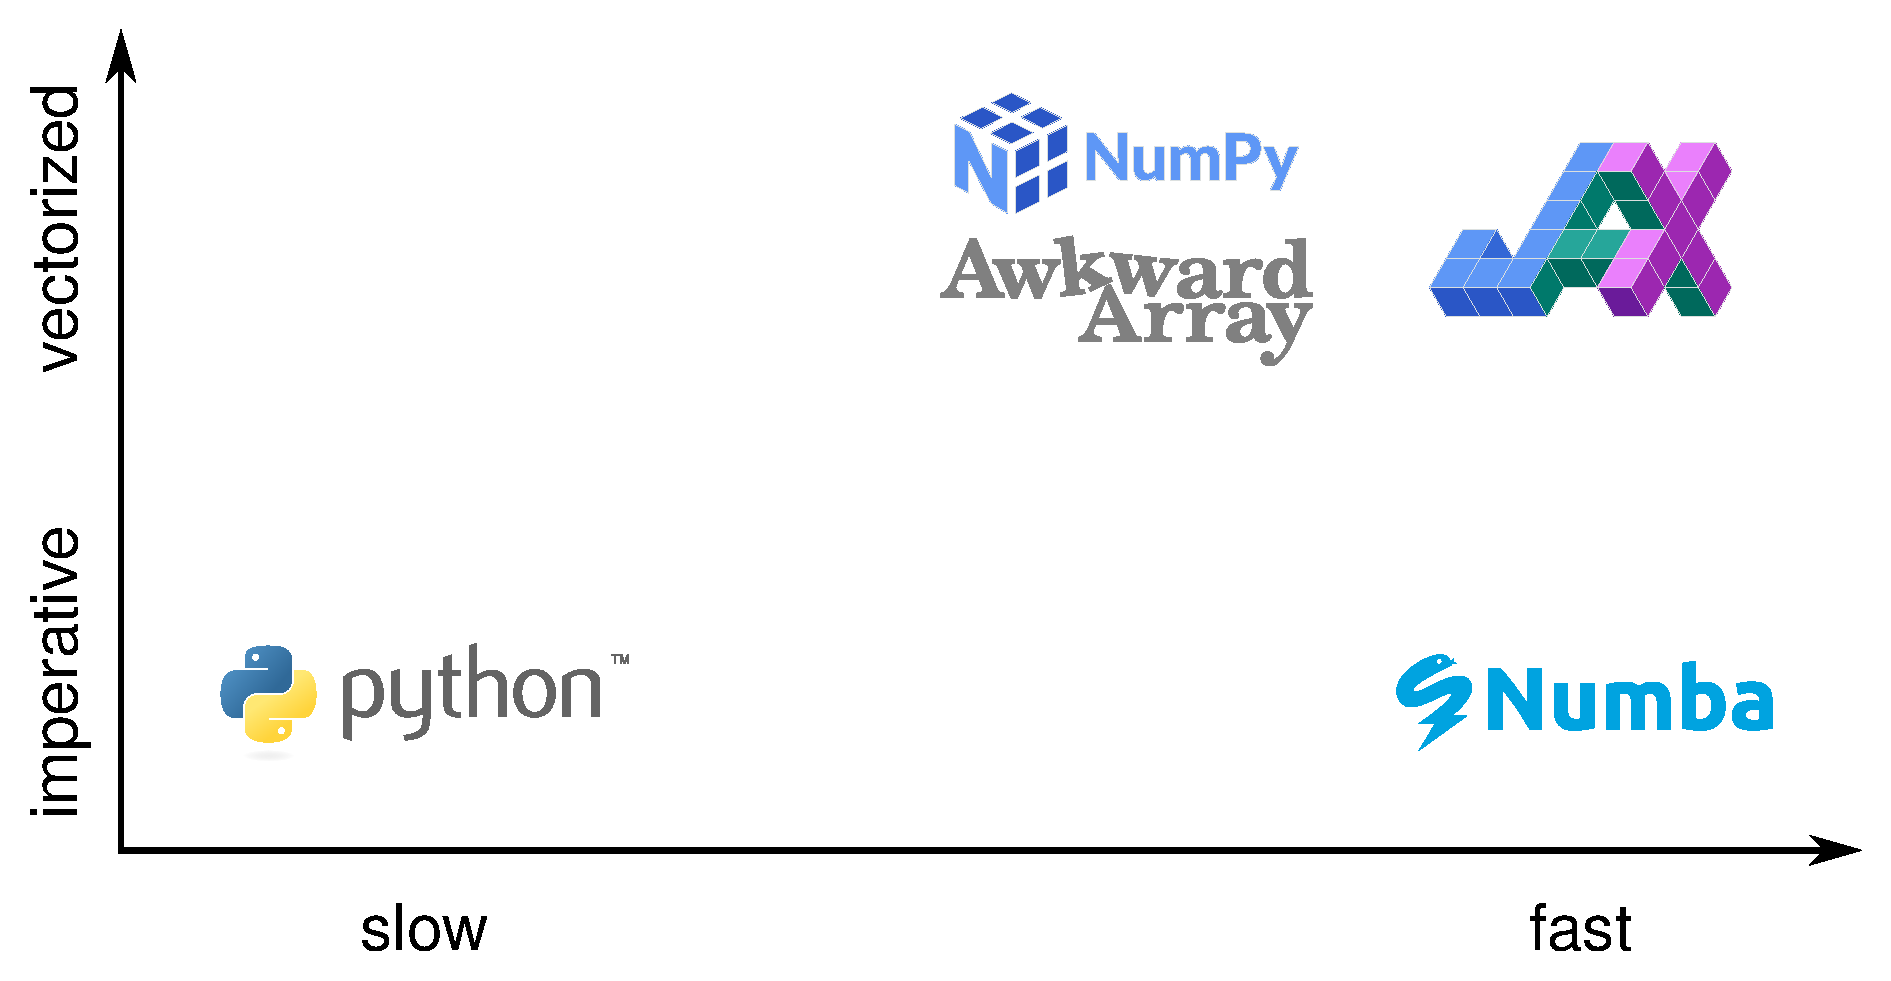
\includegraphics[width=0.9\linewidth]{img/slow-fast-imperative-vectorized.pdf}
\end{center}
\end{frame}

\begin{frame}{\mbox{ }}
\vspace{0.75 cm}
\begin{center}
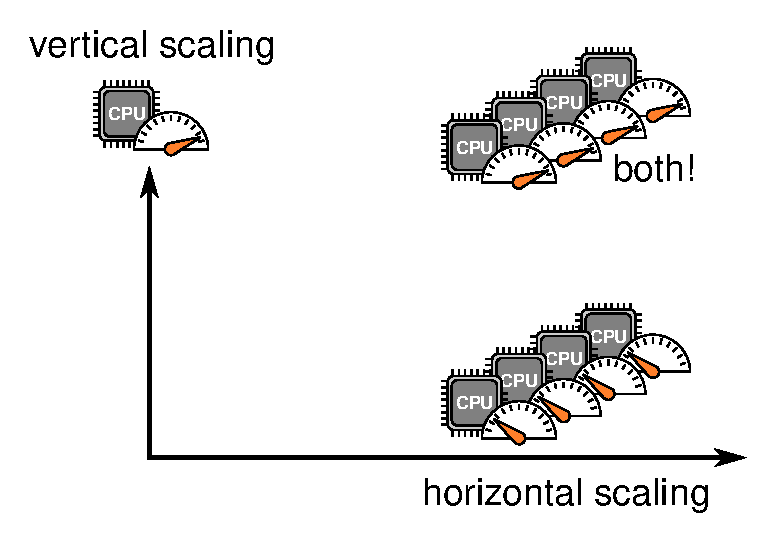
\includegraphics[width=0.6\linewidth]{img/horizontal-and-vertical-scaling.pdf}
\end{center}
\end{frame}

\begin{frame}{CERN Courier, March 1972}
\vspace{0.2 cm}
\begin{center}
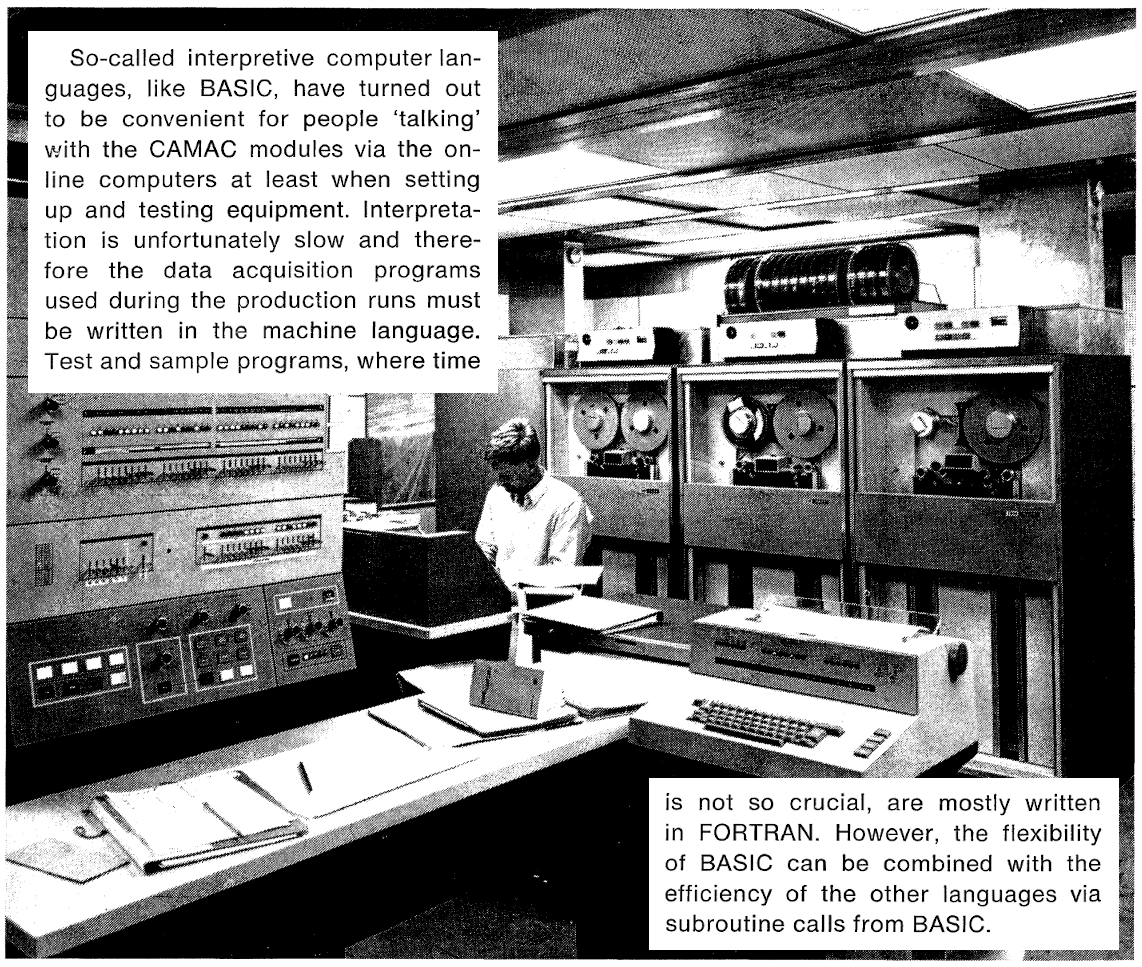
\includegraphics[width=0.65\linewidth]{img/cern-courier-basic.png}
\end{center}
\end{frame}

\begin{frame}{Lukas Taylor's summary talk at CHEP 2001}
\vspace{0.2 cm}
\begin{center}
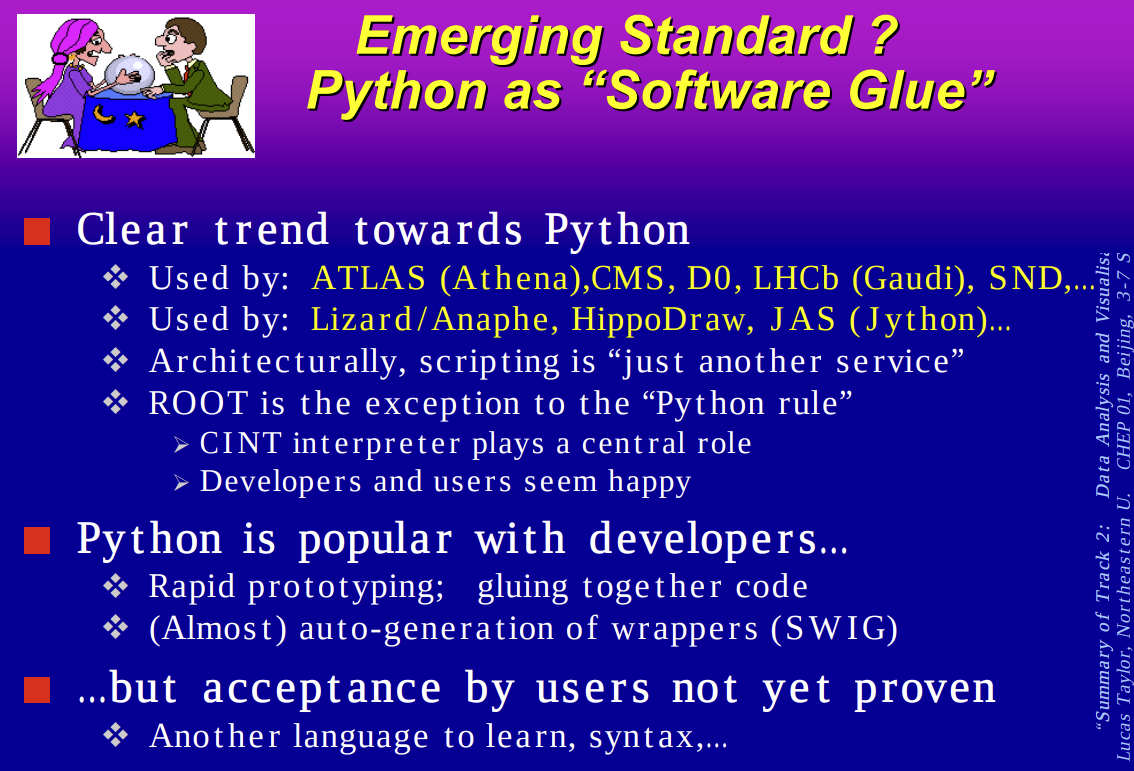
\includegraphics[width=0.8\linewidth]{img/chep-2001-python.png}
\end{center}
\end{frame}

\begin{frame}{Adoption of Python for CMS analysis}
\vspace{0.2 cm}
\begin{columns}
\column{1.15\linewidth}
\only<1>{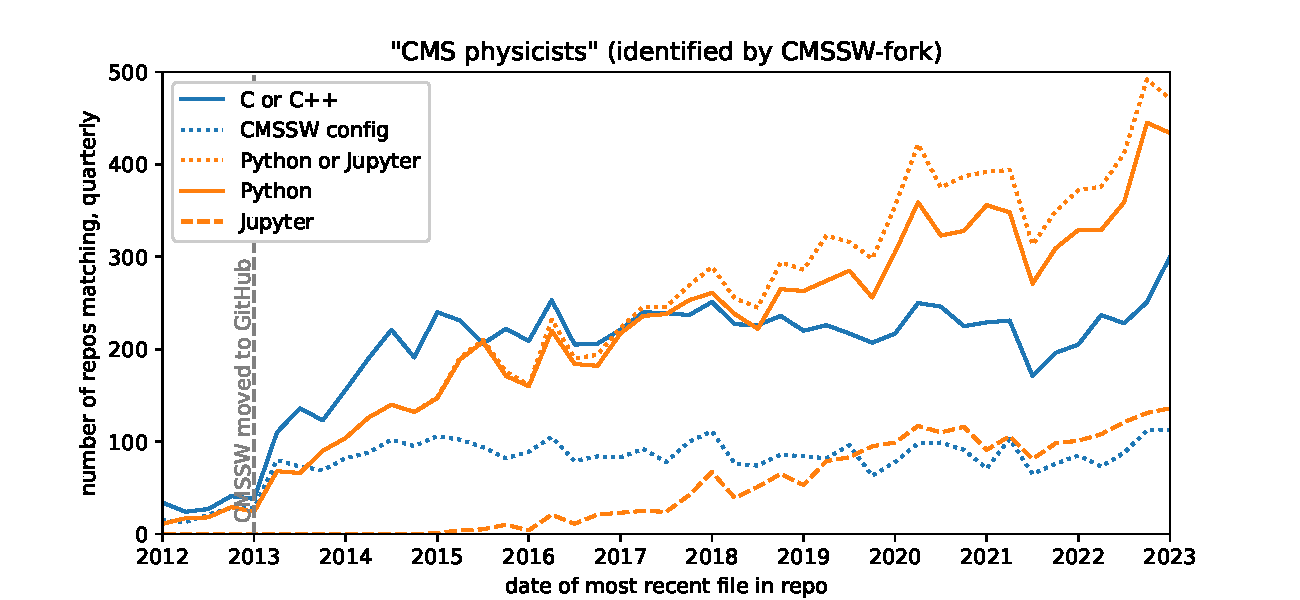
\includegraphics[width=\linewidth]{img/github-language-cmsswseed.pdf}}\only<2>{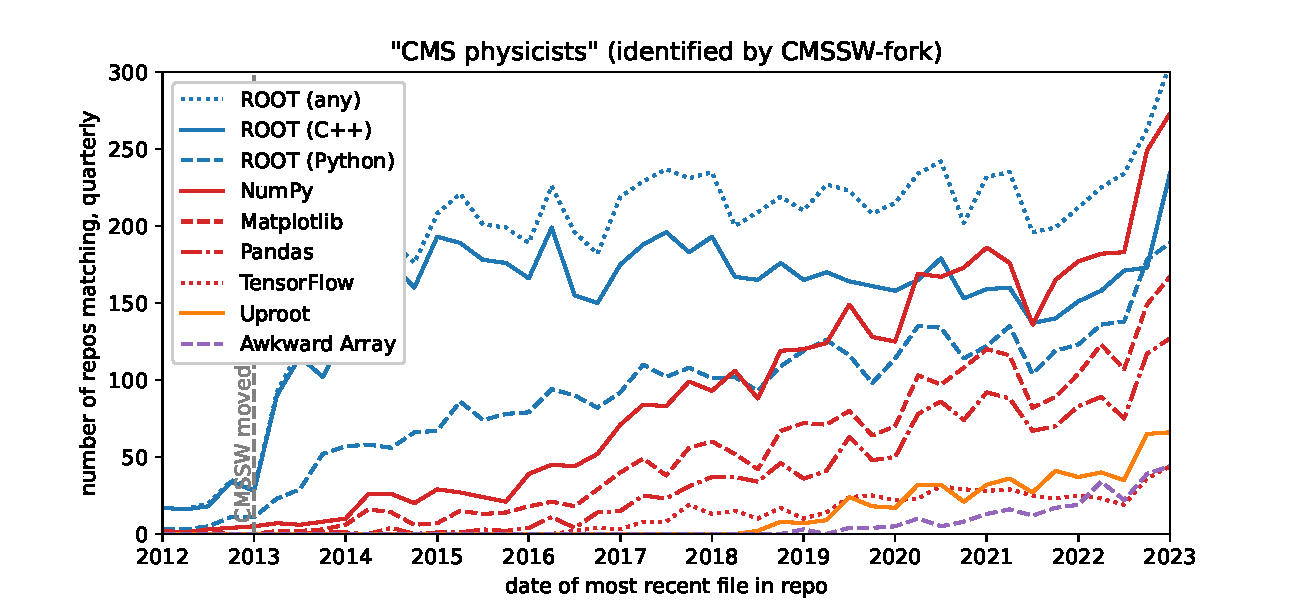
\includegraphics[width=\linewidth]{img/github-package-cmsswseed.pdf}}\only<3>{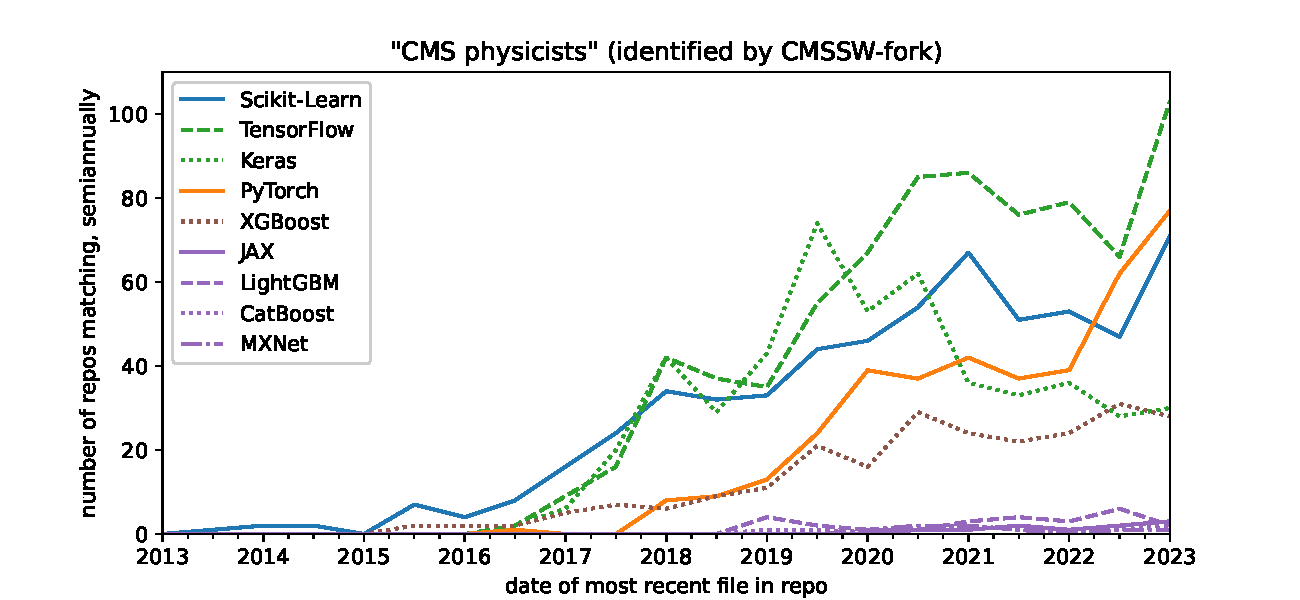
\includegraphics[width=\linewidth]{img/github-ml-package-cmsswseed.pdf}}
\end{columns}
\end{frame}

\begin{frame}{\mbox{ }}
\vspace{0.2 cm}
\begin{center}
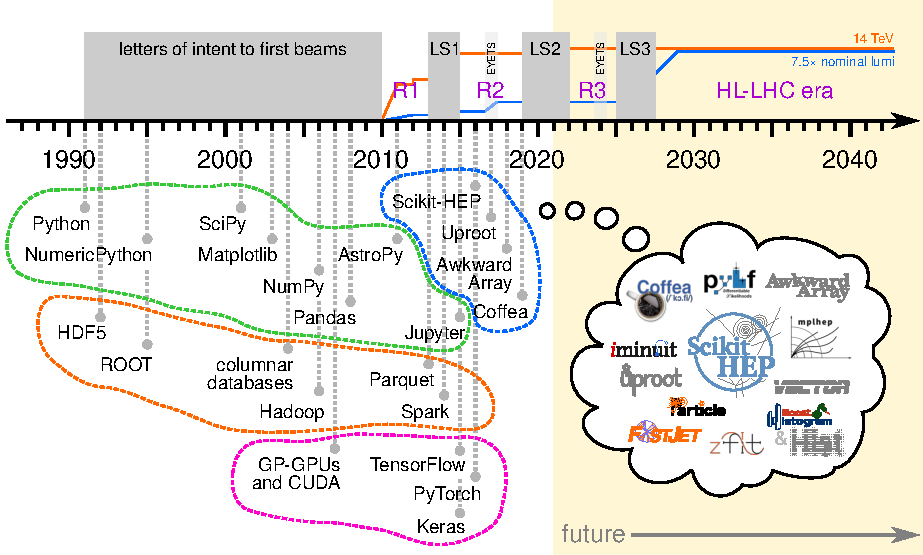
\includegraphics[width=0.9\linewidth]{img/hllhc-python-timeline-5.pdf}
\end{center}
\end{frame}

\end{document}
